% THIS DOCUMENT IS FOLLOWS THE VOLERE TEMPLATE BY Suzanne Robertson and James Robertson
% ONLY THE SECTION HEADINGS ARE PROVIDED
%
% Initial draft from https://github.com/Dieblich/volere
%
% Risks are removed because they are covered by the Hazard Analysis
\documentclass[12pt]{article}

\usepackage{booktabs}
\usepackage{tabularx}
\usepackage{enumerate} 
\usepackage{float}
\usepackage{hyperref}
\usepackage{enumerate}
\usepackage{graphicx}
\usepackage{float}
\usepackage{longtable}
\usepackage{multirow}
\hypersetup{
    bookmarks=true,         % show bookmarks bar?
      colorlinks=true,      % false: boxed links; true: colored links
    linkcolor=red,          % color of internal links (change box color with linkbordercolor)
    citecolor=green,        % color of links to bibliography
    filecolor=magenta,      % color of file links
    urlcolor=cyan           % color of external links
}

\newcommand{\lips}{\textit{Insert your content here.}}

%% Comments

\usepackage{color}

\newif\ifcomments\commentstrue %displays comments
%\newif\ifcomments\commentsfalse %so that comments do not display

\ifcomments
\newcommand{\authornote}[3]{\textcolor{#1}{[#3 ---#2]}}
\newcommand{\todo}[1]{\textcolor{red}{[TODO: #1]}}
\else
\newcommand{\authornote}[3]{}
\newcommand{\todo}[1]{}
\fi

\newcommand{\wss}[1]{\authornote{blue}{SS}{#1}} 
\newcommand{\plt}[1]{\authornote{magenta}{TPLT}{#1}} %For explanation of the template
\newcommand{\an}[1]{\authornote{cyan}{Author}{#1}}

%% Common Parts

\newcommand{\progname}{Software Engineering} % PUT YOUR PROGRAM NAME HERE
\newcommand{\authname}{Team \#22, TeleHealth Insights
\\ Mitchell Weingust
\\ Parisha Nizam
\\ Promish Kandel
\\ Jasmine Sun-Hu} % AUTHOR NAMES                  

\usepackage{hyperref}
    \hypersetup{colorlinks=true, linkcolor=blue, citecolor=blue, filecolor=blue,
                urlcolor=blue, unicode=false}
    \urlstyle{same}
                                


\begin{document}

\title{Software Requirements Specification for \progname} 
\author{\authname}
\date{\today}
	
\maketitle

~\newpage

\pagenumbering{roman}

\tableofcontents

~\newpage

\section*{Revision History}

\begin{tabularx}{\textwidth}{p{1.5cm}p{1cm}p{3.5cm}X}
\toprule {\textbf{Date}} & {\textbf{Vers.}} & {\textbf{Contributors}} & {\textbf{Notes}}\\
\midrule
10/03/24 & 1.0 & Mitchell Weingust, Parisha Nizam & Added Functional Requirements 9.1, 9.2, 9.3 \\
10/03/24 & 1.1 & Promish Kandel, Jasmine Sun-Hu & Added Functional Requirements 9.4,9.5,9.6, and sections 1,3,5\\
10/04/24 & 1.2 & Mitchell Weingust, Parisha Nizam & Added Non Functional Requirements 11, 13, 15, 17\\
10/04/24 & 1.3 & Jasmine Sun-Hu & Added Nonfunctional Requirements 10,14,16\\
10/05/24 & 1.4 & Promish Kandel & Added Nonfunctional Requirements 12\\
10/06/24 & 1.5 & Mitchell Weingust, Parisha Nizam & Added Sections 2, 4\\
10/09/24 & 1.6 & Jasmine Sun-Hu & Added Scope of the Work: Current Situation, Costs 6.1, 23\\
10/09/24 & 1.7 & Mitchell Weingust & Added Sections 8, 18\\
10/10/24 & 1.8 & Mitchell Weingust & Added Sections 8, 19\\
10/11/24 & 1.9 & Jasmine Sun-Hu & Added Section 6.4, Traceability Matrix, References\\
10/11/24 & 2.0 & Promish Kandel & Added Section 20,24,25 and Formal Specification\\
10/11/24 & 2.1 & Parisha Nizam & Added Section 21,22,26 Traceability Matrix \\
10/11/24 & 2.2 & All & Added Reflection and minor edits \\
12/24/24 & 2.3 & Jasmine Sun-Hu & Implemented Assigned Peer Feedback \\\\
\bottomrule
\end{tabularx}

~\\

~\newpage
\section{Purpose of the Project}
\subsection{User Business}
\hspace{1.5em}The project being outlined in this document is an at-home bilingual speech 
assessment system with video and audio analysis features. The system is designed 
to provide clear guidance to parents when administering the assessment to their 
children, in an environment where speech-language pathologists (SLPs) are 
unavailable. By streamlining the assessment process, the project aims to provide a 
convenient and comprehensive solution for SLPs to assess and support their patients'
speech and language development remotely. 
\subsection{Goals of the Project}
\begin{itemize}
  \item[1.2.1] \textbf{Intuitive Parent Interface:}  
  The system must provide an intuitive interface that helps parents administer 
  language assessments effectively. It should be easy to navigate with clear and 
  meaningful symbols, and it must provide real-time feedback to ensure parents are 
  aware their interactions are being processed throughout the assessment.

  \item[1.2.2] \textbf{Engaging Child Interaction:}  
  The system must feature an engaging interface for children to keep them attentive 
  during the assessment. The design should be simple yet visually appealing, using 
  colors and images to attract the child’s attention to the questions and selections,
  ensuring that children remain engaged throughout the assessment.

  \item[1.2.3] \textbf{Reliable Assessment Data for SLPs:}  
  The system must provide reliable and accurate assessment data for speech-language 
  pathologists (SLPs) by capturing additional contextual data. This includes 
  identifying background interference, signs of bias, and potential test 
  complications. The system should also filter out noise and detect multiple users 
  to prevent external guidance from affecting the assessment results.

  \item[1.2.4] \textbf{Data Security:}  
  The system must ensure that all sensitive health and personal data is securely 
  stored and accessed. It should implement a strong security protocol to securely 
  store, retrieve, and manage sensitive data, ensuring the privacy and confidentiality
  of the users.

  \item[1.2.5] \textbf{Cross-Platform Compatibility:}  
  The system must provide cross-platform compatibility, ensuring that it functions 
  seamlessly across different devices and screen sizes. It should be accessible to 
  both parents and children, rendering correctly on all screen formats, whether on 
  phones, tablets, or desktops.
\end{itemize}

\section{Stakeholders}
\subsection{Client}
  \begin{itemize}
    \item This project's client is Researcher, Clinician Assistant, Professor at the University of Southern California, Dr. Yao Du.
    \item Another stakeholder is this project's supervisor, Dr. Irene Ye Yuan, Assistant Professor in the Department of Computing and Software at McMaster University.
  \end{itemize}
  \subsection{Customer}
  \begin{itemize}
    \item This project's customers are Clinicians (SLPs) who work with children that have speech difficulties.
    \item Another one of the project's customers are the children with speech difficulties who take language assessments.
    \item Another one of the project's customers are the parents of children with speech difficulties.
  \end{itemize}
  \subsection{Other Stakeholders}
  \begin{itemize}
    \item Data Analysts may be another stakeholder, if they decide to review and analyze the data.
    \item Society is another important stakeholder to consider, as the system being developed is impactful for workers and technological developments in the healthcare field.
          As well, as this is a healthcare application, the safety of society must be taken into account to ensure the project.
          In addition, important cultural sensitivities and their appropriate contexts must be considered for the system to prevent unintentional offensiveness.
  \end{itemize}
\subsection{Hands-On Users of the Project}
\hspace{2em}Hands-on users for this project include the parents of children that have speech difficulties, as well as the children themselves, who need to take language assessments.\\
\indent In addition, speech language pathologists are important hands-on users for this project as they are assessing the assessment results, assessing children's performances, and keeping track of the children's improvements overtime. 
\subsection{Personas}
\textbf{User Profile:}\\
Name: Paul Blart\\
Age: 42\\
Job: Mall Cop\\
Personality Traits: Caring, Strict, Empathetic, Impatient, Stubborn\\

\textbf{Key Task Goals:}
\begin{itemize}
  \item Convenient access to healthcare technology for his family.
  \item Use a system that is easy for both him and his child to learn and use.
  \item Wants a system that is available for him to use at any time, as his job doesn't usually allow him to schedule in-person assessments easily.
  \item Cares about his family's safety and security, so he wants a system that will keep their healthcare and personal information confidential.  
\end{itemize}

\textbf{Motivations/Frustrations:}
\begin{itemize}
  \item Paul is motivated by caring for his child, and wants the best support for them.
  \item Paul is encouraged to find a system that his child can easily navigate, so it does not stress them out or make their lives more difficult.
  \item Paul is frustrated by systems that take too long to load.
  \item Paul is frustrated by systems that are not easy to use, as he often has to dedicate long periods of time to learn new technology.
  \item Paul doesn't like changing his routine, so he wants to find a system that works for him, and stick with it.
  \item Paul is motivated to find a system that will best help his child so he can see how their language understanding improves over time.
\end{itemize}

\textbf{Quote:}\\
'Man, technology is so hard! I love my kid, but I am so busy. My kid doesn't like going in person to speak with clinicians. I need a solution that will make them feel more comfortable. I wish there was a way to track their progress, so I can see how they're improving.'\\

\subsection{Priorities Assigned to Users}
\begin{enumerate}
  \item Children (who take learning assessments)
  \item Parents and SLPs
  \item Researcher (Dr. Yao Du)
  \item Supervisor (Dr. Irene Ye Yuan)
  \item Society
\end{enumerate}
\subsection{User Participation}
\begin{itemize}
  \item Parents
  \subitem{No input necessary.}
  \item Children (who take learning assessments)
  \subitem{No input necessary.}
  \item SLPs
  \subitem{No input necessary.}
  \item Researcher (Dr. Yao Du)
  \subitem{Occassional input, communication is managed through the project's supervisor.}
  \item Supervisor (Dr. Irene Ye Yuan)
  \subitem{Frequent input, with minimum weekly checkins to ensure the project is within scope and on-track.}
  \item Society
  \subitem{No input necessary.}
\end{itemize}

\subsection{Maintenance Users and Service Technicians}
N/A\\

\section{Mandated Constraints}
\subsection{Solution Constraints}
\begin{itemize}
  \item[3.1.1] The platform must be accessible as a website to provide ease of access to users without requiring special software installations.
  \item[] Rationale: A web-based platform maximizes accessibility for users across various devices, and prevents installation of external software which could be a barrier of entry.
  \item[] Fit Criterion: The platform must run without requiring the installation of external software, and display with visual consistency across at least 3 different browsers.
  \item[3.1.2] The platform must adhere to HIPAA or relevant data protection regulations to ensure patient data privacy and security \cite{hipaa}.
  \item[] Rationale: Compliance with HIPAA will maintain trust that sensitive data is protected for patients and users of the website.
  \item[] Fit Criterion: A HIPAA compliance audit must confirm data encryption, user authentication and data storage adhere to HIPAA
  \item[3.1.3] Access to the platform must be restricted to authorized users, with secure authentication processes in place.
  \item[] Rationale: This ensures data privacy and prevents data breaches from unauthorized users.
  \item[] Fit Criterion: The platform must require secure authentication of all users, and testing must confirm there are no unauthorized access vulnerabilities found before deployment.
  \item[3.1.4] The system must be capable of scaling to accommodate an increasing number of users and growing data storage needs as the client expands.
  \item[] Rationale: Scalability ensures the system can handle future growth without degrading performance
  \item[] Fit Criterion: Load testing must demonstrate the system can support 200 concurrent users without performance degradation
  \item[3.1.5] The platform must support assessment sessions of up to at least 30 minutes to align with standard telehealth consultation times.
  \item[] Rationale: Telehealth sessions often last for extended periods of time, the platform should maintain uninterrupted functionality.
  \item[] Fit Criterion: System testing must confirm that the platform can maintain video and audio recordings for at least 30 minutes without any interruptions or crashes.
  \item[3.1.6] The platform must support adaptable video and audio quality based on internet bandwidth, ensuring clarity and reliability during assessments.
  \item[] Rationale: A smooth and consistent performance improves user experience.
  \item[] Fit Criterion: Testing must confirm that video and audio streams automatically adjust quality within a bandwidth range of 0.5 Mbps to 5 Mbps without freezing or loss of synchronization.
  \item[3.1.7] The platform must comply with WCAG 2.1 accessibility standards, making it accessible to users with varying needs \cite{wcag}.
  \item[] Rationale: The project is focused around children with speech difficulties, meeting accessibility standards is necessary to ensure the platform is usable by the user base.
  \item[] Fit Criterion: A WCAG compliance audit must confirm adherence to at least Level AA standards.
  \item[3.1.8] Patient records must be retained for a minimum of 7 years from the last visit or at least 1 year after the patient turns 18, whichever is 
  longer, in accordance with California law \cite{californialaw}.
  \item[] Rationale: Keeping records for the specified duration ensures compliance with legal obligations and supports continuous care.
  \item[] Fit Criterion: System audits must confirm patient records are kept for the required amount of time and the data can be archived securely beyond the active period
\end{itemize}
\subsection{Implementation Environment of the Current System}
\begin{itemize}
  \item[3.2.1] The platform’s hosting environment must meet HIPAA-compliance standards to ensure data security \cite{hipaa}.
  \item[] Rationale: A compliant hosting environment is important for protecting sensitive data.
  \item[] Fit Criterion: An infrastructure compliance review must confirm that the hosting environment meets encryption, access control, and logging requirements for HIPAA.
  \item[3.2.2] The development framework must support scalable, secure, and efficient web application development, compatible with existing technical 
  infrastructure.
  \item[] Rationale: A compatible framework is important to ensure scalability and security, and also reduces technical overhead.
  \item[] Fit Criterion: The website must achieve a response time of less than 300ms for 95\% of requests and pass security evaluations with no more than one low severity vulnerability identified during testing.
\end{itemize}
\subsection{Partner or Collaborative Applications}
\begin{itemize}
  \item[3.3.1] The platform must be capable of exporting data as an Excel file, allowing for easy sharing, analysis, and compatibility with other systems
  that clinicians may use for data processing.
  \item[] Rationale: Universally accepted format files make any integration with third party systems and enables flexible data handling.
  \item[] Fit Criterion: Testing must confirm that exported files retain all data fields and formatting accurately when opened in Excel.
\end{itemize}
\subsection{Off-the-Shelf Software}
\begin{itemize}
  \item[3.4.1] N/A. There are no mandated off-the-shelf software constraints. 
\end{itemize}
\subsection{Anticipated Workplace Environment}
\begin{itemize}
  \item[3.5.1] The platform must be compatible across a range of devices, including desktops, tablets, and mobile phones.
  \item[] Rationale: Device compatibility ensures users can access the platform from their preferred device, enhancing accessibility and convenience.
  \item[] Fit Criterion: Testing must confirm that the platform is fully functional and displays correctly on devices with screen sizes ranging from 4” to 27”.
\end{itemize}
\subsection{Schedule Constraints}
\begin{itemize}
  \item[3.6.1] The proof-of-concept shall be complete and demonstrated between Nov. 11-22, 2024.
  \item[] Rationale: Required by the Capstone course instructors.
  \item[] Fit Criterion: Proof-of-concept must be operational and ready for demonstration by Nov. 11, 2024.
  \item[3.6.2] Revision 0 of the project shall be complete and demonstrated between February 3-14, 2025.
  \item[] Rationale: Required by the Capstone course instructors.
  \item[] Fit Criterion:  Revision 0 must incorporate feedback and meet all baseline requirements by February 3, 2025.
  \item[3.6.3] The final product shall be complete and demonstrated between March 24-30, 2025.
  \item[] Rationale: Required by the Capstone course instructors.
  \item[] Fit Criterion: The final product must be operational and meet all specifications, verified through testing and stakeholder acceptance by March 24, 2025
\end{itemize}
\subsection{Budget Constraints}
\begin{itemize}
  \item[3.7.1] The project budget must not exceed \$750 CAD. 
  \item[] Rationale: Staying within budget ensures the project remains financially feasible.
  \item[] Fit Criterion: Financial tracking must confirm that total expenses do not exceed \$750 CAD throughout the project lifecycle.
\end{itemize}
\subsection{Enterprise Constraints}
\begin{itemize}
  \item[3.8.1] N/A. There are no mandated enterprise constraints.
\end{itemize}

\section{Naming Conventions and Terminology}
\subsection{Glossary of All Terms, Including Acronyms, Used by Stakeholders
involved in the Project}

\begin{table}[h!]
\begin{tabularx}{\textwidth}{p{2cm}X}
  \toprule {\textbf{Terms}} & {\textbf{Definition}}\\
  \midrule
  SLP & Speech Language Pathologist\\
  HIPAA & Health Insurance Portability and Accountability Act \cite{hipaa}\\
  WCAG & Web Content Accessibility Guidelines \cite{wcag}\\
  ML & Machine Learning\\
  PUC & Product Use Case\\
  FR & Functional Requirement\\
  NFG & Non-Functional Requirement\\
  BUC & Business Use Case\\
  TB & Terabyte\\
  \bottomrule
\end{tabularx}
\caption{Naming Conventions and Terminology}
\end{table}

\section{Relevant Facts And Assumptions}
\subsection{Relevant Facts}
\begin{itemize}
  \item[5.1.1] The project is subject to healthcare privacy laws like HIPAA, ensuring that patient data is securely stored and managed \cite{hipaa}.
  \item[5.1.2] The client has requested a web-based platform, indicating a preference for accessibility without the need for specialized 
  software installations.
  \item[5.1.3] The platform will have two primary user roles. The clinicians who perform assessments and review results and the parents who 
  administer the assessment to their children who are the patients.
\end{itemize}
\subsection{Business Rules}
\begin{itemize}
  \item[5.2.1] Only authorized users (clinicians) can access patient data.
  \item[5.2.2] Patient records must be retained for at least 7 years from the last visit, or 1 year after the patient turns 18, whichever is longer, 
  to comply with California state law.
  \item[5.2.3] The platform must comply with WCAG 2.1 to ensure it is accessible to users with disabilities \cite{wcag}.
  \item[5.2.4] All patient data must be encrypted both in transit and at rest to maintain confidentiality and meet regulatory standards.
  \item[5.2.5] The platform must generate reports based on assessment data, which can be reviewed and stored within the system 
  \item[5.2.6] Video and audio recordings must automatically adjust to optimize based on internet bandwidth, ensuring quality without excessive 
  buffering or latency.
\end{itemize}
\subsection{Assumptions}
\begin{itemize}
  \item[5.3.1] All users of the system have reliable internet connections that can support uploading video and audio recordings to the database.
  \item[5.3.2] All patient data will be stored on servers located in regions that comply with healthcare data residency regulations.
  \item[5.3.3] The platform is assumed to be accessible from various devices with working microphone and camera, though it may perform optimally on 
  desktops.
  \item[5.3.4] Assessments will not exceed 30 minutes per session to fit standard telehealth assessment times.
  \item[5.3.5] It is assumed that users (both clinicians and patients) have a basic level of comfort with using web applications and online 
  communication tools.
  \item[5.3.6] The platform may need to accommodate additional users and storage demands as the client scales its telehealth services over time.
\end{itemize}

\section{The Scope of the Work}
\subsection{The Current Situation}
\hspace{1.5em}Currently, speech language assessments for bilingual children with speech difficulties require in-person visits, which can be logistically challenging 
for families and clinicians. While there are some existing telehealth solutions, they are much more generalized and there are no existing solutions 
specifically for the unique needs of bilingual children with speech difficulties such as a platform that offers assessments in multiple languages. 
There is a need for a remote online solution where parents can administer language assessments to their children while minimizing the bias the parent 
may introduce during the assessment. \\\\
\indent Additionally, clinicians currently store all unprocessed data on excel files which can be tedious, disorganized, and require extra time from the clinician 
to go through. A solution that tracks the remote assessment responses and generates a report from processed data will save the clinician or SLP significant 
time. Moreover, a solution that tracks the interactions between the user and the interface which can detect points of bias or disturbance can help a clinician 
review an assessment session and either accept the remote assessment results with confidence or recognize where points of bias occur.

\subsection{The Context of the Work}
\hspace{1.5em}The diagram below models the high level interactions within the system as well as with any external systems.
\begin{figure}[H]
  \centering
  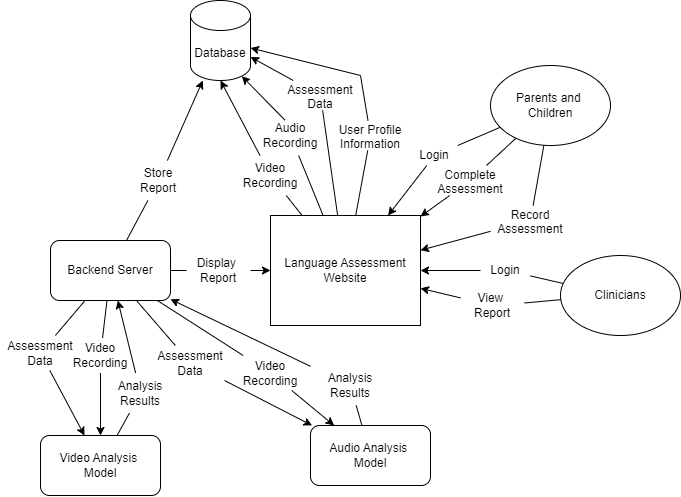
\includegraphics[scale=0.7]{images/ContextoftheWork.png}
  \caption{Context of the Work}
\end{figure}

All incoming and outgoing data to and from the database will be processed through the backend server first, the arrows are drawn directly for a simpler high-level diagram. 
\subsection{Work Partitioning}
\begin{table}[H]
  \centering
  \begin{tabularx}{1.2\textwidth} { 
     >{\raggedright\arraybackslash}X 
    | >{\raggedright\arraybackslash}X 
    | >{\raggedright\arraybackslash}X  }
  \toprule
  \textbf{Event Name} & \textbf{Input/Output} & \textbf{Summary} \\
  \midrule
  Provide Display Report & IN: Display Report & Give a report of all sessions\\ 
  \midrule
  Provide Assessmenet answer & IN: Completed Assessment & Give a list of all the answers picked for a current session assessment \\ 
  \midrule
  Provide Record Assessmenet & IN: Record Assessmenet & Give a video recording taken form the current assessment \\ 
  \midrule
  Display Report & OUT: View Report  & Display report for all sessions when requested by clinician   \\ 
  \midrule
  Store Video Recording & OUT: Video Recording  & Send video recording to be stored in the database \\
  \midrule
  Store Audio Recording & OUT: Audio Recording  & Send audio recoridng to be stored in the database \\
  \midrule
  Store Assessmenet Data & OUT: Assessmenet Data  & Send assessment data for the current session to be stored in the database \\
  \midrule
  Store User Profile Information& OUT: User Profile Information  & Send user profile information for the current user to be stored in the database \\
  \midrule
  Store Report Infromation & OUT: Store Report  & Send report information with timestamps to be stored in the database \\
\bottomrule
\end{tabularx}
\end{table}
\newpage
\noindent \textbf{Work partitioning continued}
\begin{table}[H]
  \centering
  \begin{tabularx}{1.2\textwidth} { 
     >{\raggedright\arraybackslash}X 
    | >{\raggedright\arraybackslash}X 
    | >{\raggedright\arraybackslash}X  }
  \toprule
  \textbf{Event Name} & \textbf{Input/Output} & \textbf{Summary} \\
  \midrule
  Do Video Analysis & IN: Assessmenet Data, Video Recording/ OUT: Analysis Results  & Given assessmenet data and video recording, analyze the data and send the results back\\
  \midrule
  Do Audio Analysis & IN: Assessmenet Data, Video Recording/OUT: Analysis Results & Given assessment data and video recorind, analyze the data and send the results back \\
\bottomrule
\end{tabularx}
\caption{Work Partitioning of BUC}
\end{table}
\subsection{Specifying a Business Use Case (BUC)}
The following is a sequence diagram for the Video Analysis process. The business use case will be triggered by the user interacting with the system 
when they submit an assessment. The output will be the video analysis detecting and identifying any disturbances during the 
assessment and details such as the related assessment question, answer, and timestamp.

\begin{figure}[H]
  \centering
  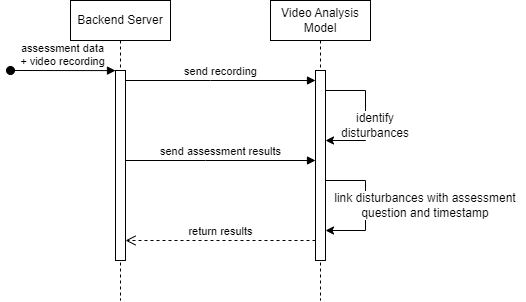
\includegraphics[scale=0.5]{images/BUC.png}
  \caption{BUC Video Analysis Sequence Diagram}
\end{figure}

\section{Business Data Model and Data Dictionary}
\subsection{Business Data Model}
\begin{figure}[H]
  \centering
  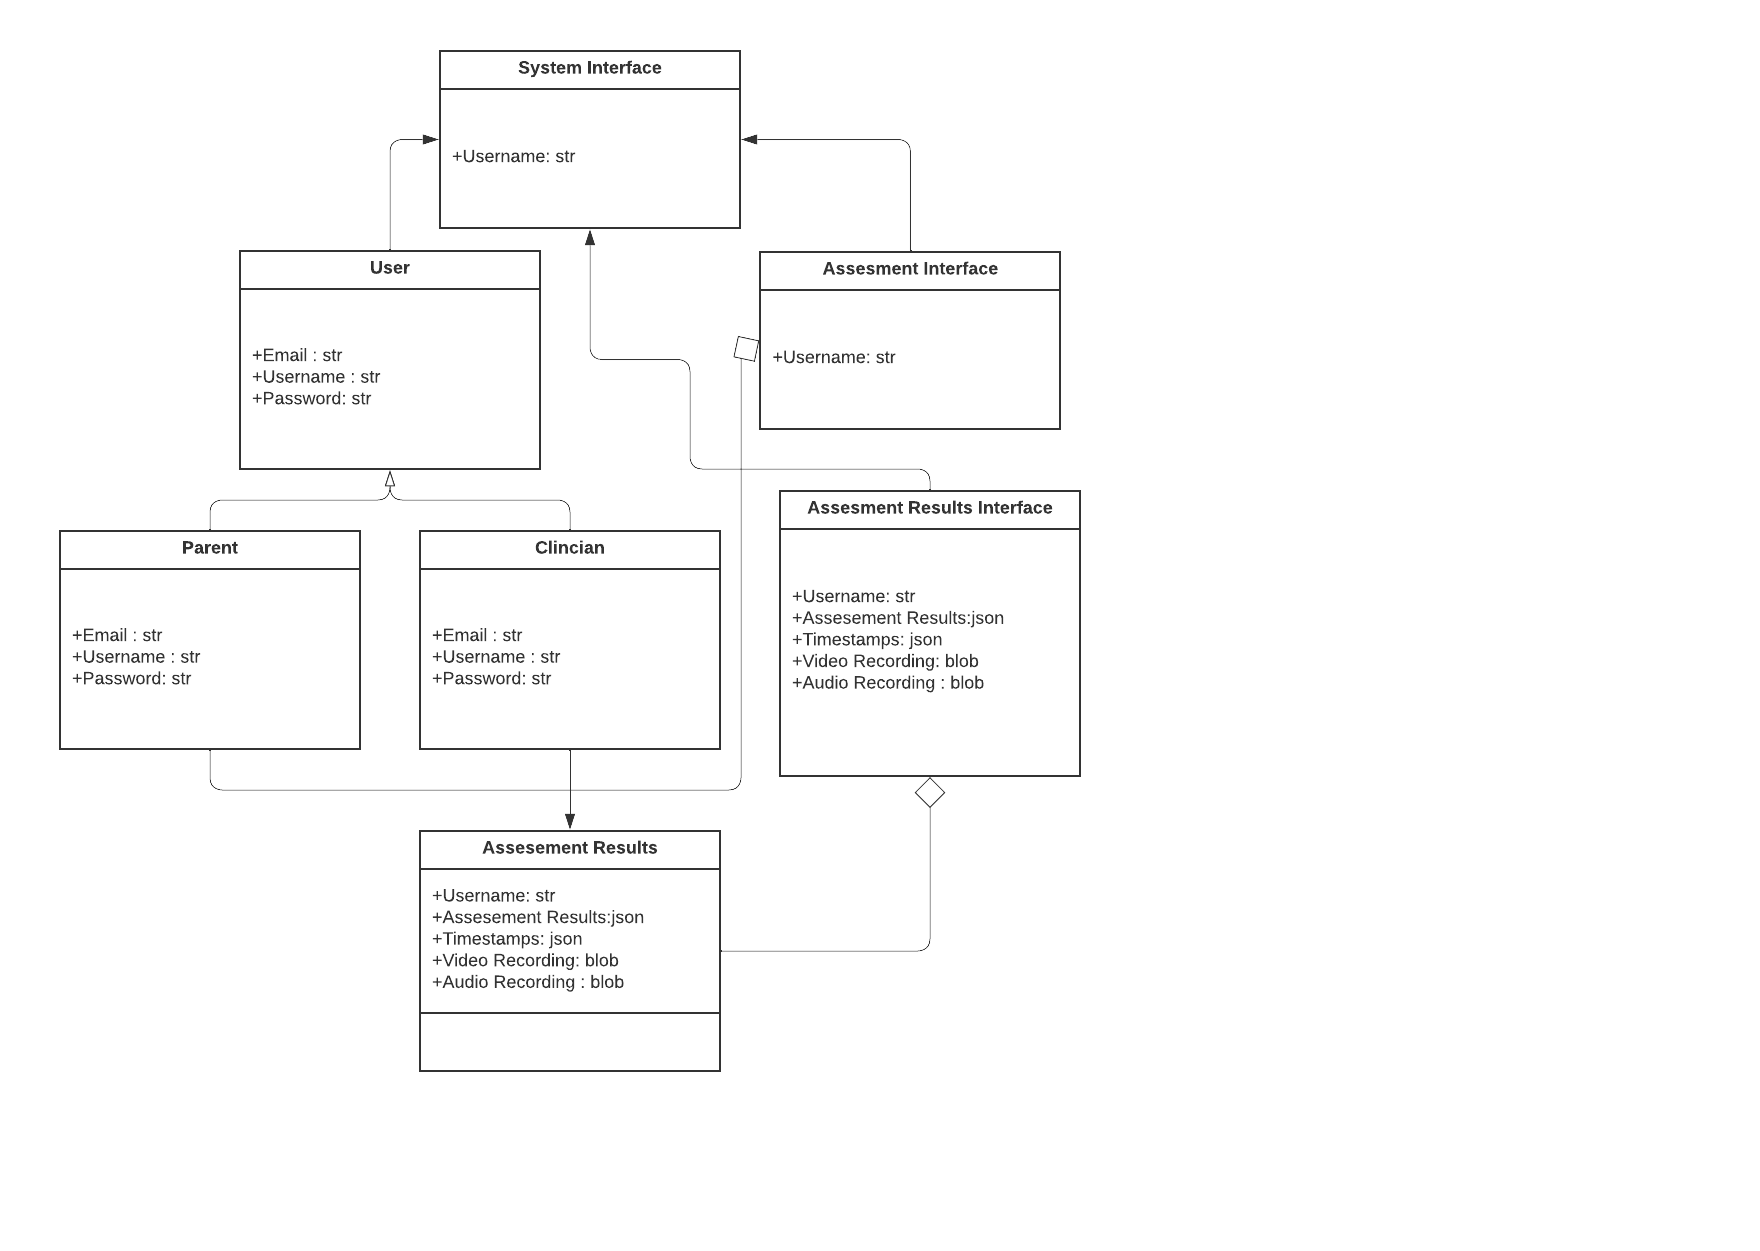
\includegraphics[scale=0.35]{images/UML class.png}
  \caption{UML Diagram of System's Data Layout}
\end{figure}
\subsection{Data Dictionary}
\begin{table}[h!]
\begin{tabularx}{\textwidth}{p{2.5cm}p{3cm}X}
  \toprule {\textbf{Name}} & {\textbf{Type}} & {\textbf{Content}}\\
  \midrule
  System Interface & Interface & Encompasses entire system that a user can view, using username \\ 
  \hline
  User & Parent Class & User Content \\ 
  \hline 
  Parent & Class & Parent Content \\ 
  \hline
  Clinician & Clinician Class & Clinician Content \\ 
  \hline 
  Email & Attribute & Login email \\
  \hline 
  Username & Attribute & Unique Login Username \\
  \hline 
  Password & Attribute & Unique Password \\
  \hline 
  Assessment Results & Class & Stores Result data from assessments \\
  \hline 
  Assessment Results & Attribute & Stores data from assessment questions (selected answers and results) in a json \\
  \hline 
  Timestamps & Attribute & Stores timestamp data at each question starting point in a json \\
  \hline 
  Video Recording & Attribute & Video Recordings of assessment is stored as blob \\
  \hline 
  Audio Recording & Attribute & Audio Recordings of assessment is stored as blob \\
  \hline 
  Assessment Results Interface & Interface & Stores assessment data and displays to clinicians \\ 
  \hline 
  Assessment Interface & Interface & Displays view for parent to learn, and complete assessment with child \\
  \bottomrule
  \end{tabularx}
  \caption{Descriptions of Data Elements in Model}
\end{table}

\section{The Scope of the Product}
\subsection{Product Boundary}
\begin{figure}[H]
  \centering
  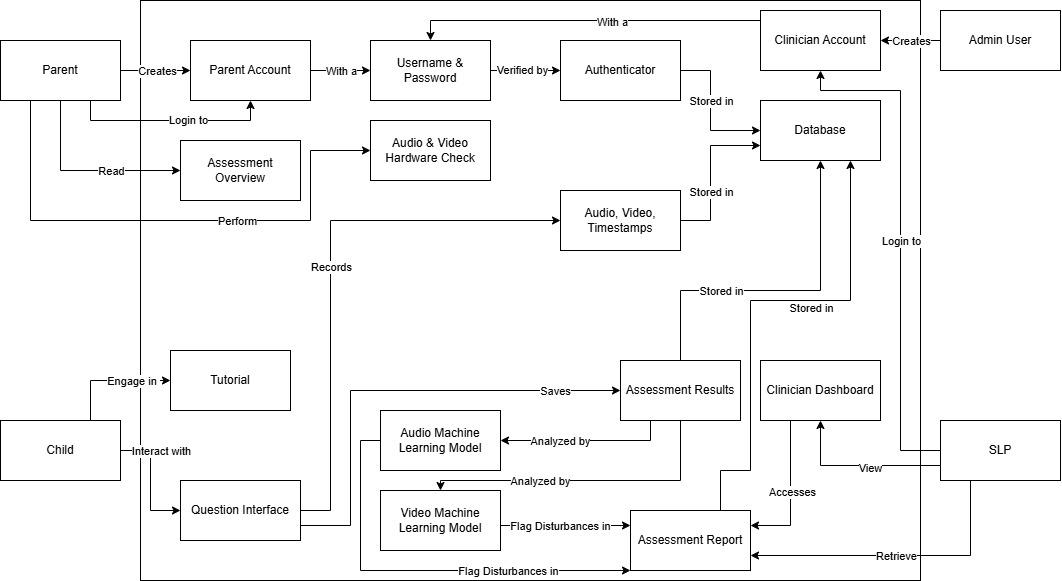
\includegraphics[scale=0.45]{images/BoundaryDiagram.jpg}
  \caption{Boundary Diagram}
\end{figure}
\begin{figure}[H]
  \centering
  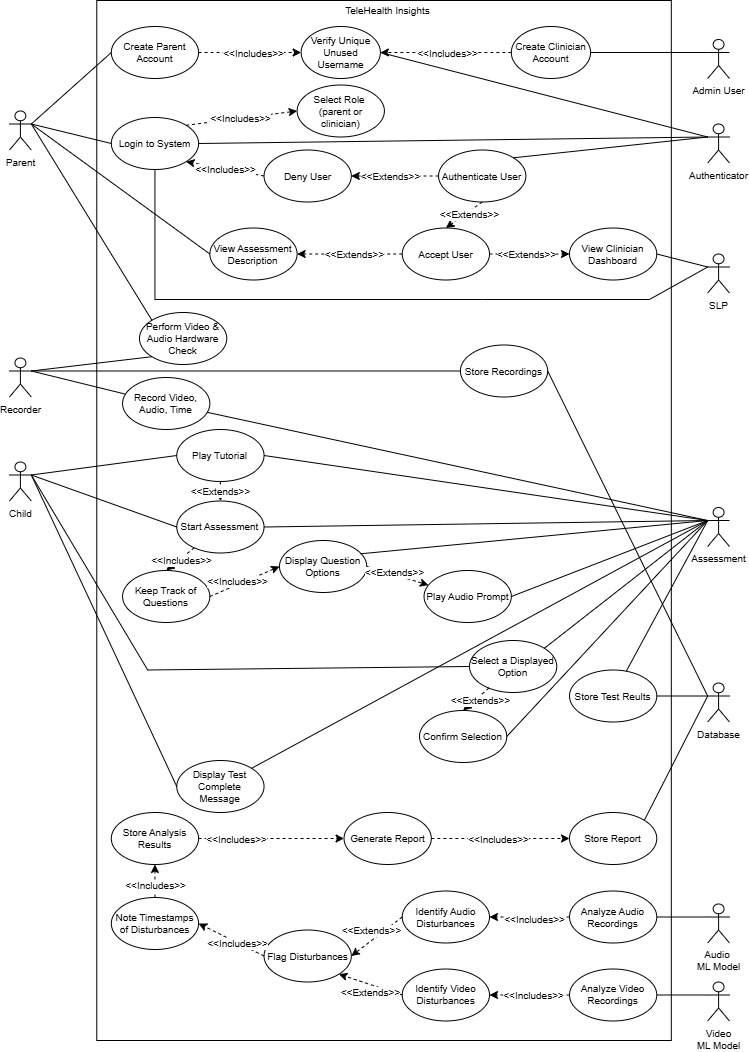
\includegraphics[scale=0.5]{images/UseCaseDiagram.jpg}
  \caption{User Case Diagram}
\end{figure}
\subsection{Product Use Case Table}
\begin{longtable}{|p{2cm}|p{3.2cm}|p{3.2cm}|p{3cm}|p{3cm}|}
  \toprule {\textbf{PUC No.}} & {\textbf{PUC Name}} & {\textbf{Actor(s)}} & {\textbf{Input(s)}} & {\textbf{Output(s)}} \\
  \midrule
  PUC-01 & Create Parent Account & Parent & Username \& Password & \\
  \hline
  PUC-02 & Verify Unique Unused Username & Parent \& Authenticator & Username & Account Created or Failure Message\\
  \hline
  PUC-03 & Create Clinician Account & Admin User \& Authenticator & Username \& Password & \\
  \hline
  PUC-04 & Login to System & Parent \& Authenticator \& SLP & Username \& Password & \\
  \hline
  PUC-05 & Select Role & Parent \& SLP & Role Selection & \\
  \hline
  PUC-06 & Deny User & Parent \& Authenticator \& SLP & & Login failure message\\
  \hline
  PUC-07 & Authenticate User & Authenticator & Username \& Password & \\
  \hline
  PUC-08 & Accept User & Authenticator & & Go to View Assessment Description or View Clinician Dashboard\\
  \hline
  PUC-09 & View Assessment Description & Parent & & Display Assessment Description\\
  \hline
  PUC-10 & View Clinician Dashboard & SLP & & Display Clinician Dashboard\\
  \hline
  PUC-11 & Perform Video \& Audio Hardware Check & Parent \& Recorder & Sound Input \& Video Input & Confirmation Message or Repeat Procedure\\
  \hline
  PUC-12 & Store Recordings & Recorder \& Database & Audio Recordings \& Video Recordings & \\
  \hline
  PUC-13 & Record Video, Audio, Time & Recorder \& Assessment & Video Recordings \& Audio Recordings \& Timer & \\
  \hline
  PUC-14 & Play Tutorial & Child \& Assessment & Click Play Tutorial Button & Plays Tutorial\\
  \hline
  PUC-15 & Start Assessment & Child \& Authenticator & Click Start Assessment Button & Go to First Question\\
  \hline
  PUC-16 & Keep Track of Questions & Assessment & Click Confirm Selection& Question Number\\
  \hline
  PUC-17 & Display Question Options & Assessment & & Display Options\\
  \hline
  PUC-18 & Play Audio Prompt & Assessment & & Plays Audio\\
  \hline
  PUC-19 & Select a Displayed Option & Child \& Assessment & Select Option & Highlight Option\\
  \hline
  PUC-20 & Confirm Selection & Child \& Assessment & Select Confirm Selection & Go to Next Question or Test Complete\\
  \hline
  PUC-21 & Display Test Complete Message & Child \& Assessment & Select final Confirm Selection & Display Message\\
  \hline
  PUC-22 & Store Test Results & Assessment \& Database & Test Results & Store Results\\
  \hline
  PUC-23 & Analyze Audio Recordings & Audio ML Model & Audio Recording & Analyzed Recording Data\\
  \hline
  PUC-24 & Identify Audio Disturbances & Audio ML Model & Analyzed Recording Data & List of disturbances\\
  \hline
  PUC-25 & Analyze Video Disturbances & Video ML Model & Video Recording & Analyzed Recording Data\\
  \hline
  PUC-26 & Identify Video Disturbances & Video ML Model & Analyzed Recording Data & List of disturbances\\
  \hline
  PUC-27 & Flag Disturbances & Audio ML Model \& Video ML Model & List of disturbances & Timestamp Markers\\
  \hline
  PUC-28 & Note Timestamp of Disturbance & Audio ML Model \& Video ML Model & Timestampe Markers & Report Data\\
  \hline
  PUC-29 & Store Analysis Results & Audio ML Model \& Video ML Model \& Database & Report Data & Analaysis Results\\
  \hline
  PUC-30 & Generate Report & Database & Analysis Results & Assessment Report\\
  \hline
  PUC-31 & Store Report & Database & Assessment Report & Store Report\\
  \bottomrule
  \caption{Summary of TeleHealth System's Use Cases}
\end{longtable}
\subsection{Individual Product Use Cases (PUC's)}
\begin{enumerate}[{PUC-}01. ]
  \item Create Parent Account\\
  \textbf{Precondition: }None\\
  \textbf{Trigger: }Parent selects 'Create Account'\\
  \textbf{Outcome: }Parent is brought to screen to Create Account with their information\\
  \textbf{Postcondition: } Parent's account creation is passed to authenticator to be verified\\
\end{enumerate}

\begin{enumerate}[{PUC-}02. ]
  \item Verify Unique Unused Username\\
  \textbf{Precondition: }Parent or Admin user creates a new account\\
  \textbf{Trigger: }User types in their preferred account username for creating their account\\
  \textbf{Outcome: }
  \begin{itemize}
  \item User's account is created
  \item User needs to select a unique username
  \end{itemize}
  \textbf{Postcondition: }User is logged into their newly created account\\
\end{enumerate}

\begin{enumerate}[{PUC-}03. ]
  \item Create Clinician Account\\
  \textbf{Precondition: }Clinician goes to their admin user to request account creation\\
  \textbf{Trigger: }Admin user creates a new clincian account\\
  \textbf{Outcome: }Clinician's account creation is verified by authenticator\\
  \textbf{Postcondition: }Clinician's account is created\\
\end{enumerate}

\begin{enumerate}[{PUC-}04. ]
  \item Login to System\\
  \textbf{Precondition: }User is on login screen\\
  \textbf{Trigger: }User selects login button from home screen\\
  \textbf{Outcome: }
  \begin{itemize}
    \item User logs into their account
    \item Authenticator denies user (incorrect credentials)
  \end{itemize}
  \textbf{Postcondition: }User enters system logged into their account\\
\end{enumerate}

\begin{enumerate}[{PUC-}05. ]
  \item Select Role\\
  \textbf{Precondition: }User is on login screen\\
  \textbf{Trigger: }User selects their role (choosing between parent or clinician)\\
  \textbf{Outcome: }User's permissions are set depending on chosen role\\
  \textbf{Postcondition: }Role is selected for login\\
\end{enumerate}

\begin{enumerate}[{PUC-}06. ]
  \item Deny User\\
  \textbf{Precondition: }Authenticator could not authenticate user with their credentials\\
  \textbf{Trigger: }User entered incorrect credentials for their account\\
  \textbf{Outcome: }User is returned to the login screen\\
  \textbf{Postcondition: }User is denied entry into their account\\
\end{enumerate}

\begin{enumerate}[{PUC-}07. ]
  \item Authenticate User\\
  \textbf{Precondition: }User attempted to login to their account\\
  \textbf{Trigger: }User entered their login information on login screen\\
  \textbf{Outcome: }Authenticator verifies against account details stored in system\\
  \textbf{Postcondition: }
  \begin{itemize}
    \item If user input correct credentials, user is accepted
    \item If user input incorrect credentials, user is denied
  \end{itemize}
\end{enumerate}

\begin{enumerate}[{PUC-}08. ]
  \item Accept User\\
  \textbf{Precondition: }User login information has been verified by the Authenticator\\
  \textbf{Trigger: }User successfully inputs correct account information\\
  \textbf{Outcome: }
  \begin{itemize}
    \item If user is a clinician, user is brought to clinician dashboard
    \item If user is a parent, user is brought to view assessment description and details
  \end{itemize}
\textbf{Postcondition: }User is logged into their account in the system\\
\end{enumerate}

\begin{enumerate}[{PUC-}09. ]
  \item View Assessment Description\\
  \textbf{Precondition: }User successfully logs into the system as a parent\\
  \textbf{Trigger: }User is verified by the authenticator upon logging in\\
  \textbf{Outcome: }Assessment description details are displayed on screen\\
  \textbf{Postcondition: }User goes to assessment description screen\\
\end{enumerate}

\begin{enumerate}[{PUC-}10. ]
  \item View Clinician Dashboard\\
  \textbf{Precondition: }User successfully logs into the system as a clinician\\
  \textbf{Trigger: }User is verified by the authenticator upon logging in\\
  \textbf{Outcome: }Clinician dashboard is displayed on screen\\
  \textbf{Postcondition: }User goes to clinician dashboard screen\\
\end{enumerate}

\begin{enumerate}[{PUC-}11. ]
  \item Perform Video \& Audio Hardware Check\\
  \textbf{Precondition: }Parent read over the assessment details\\
  \textbf{Trigger: }Parent selects setup video and audio hardware check\\
  \textbf{Outcome: }Parent performs video and audio hardware check\\
  \textbf{Postcondition: }Prompt to 'go to tutorial' is displayed on screen\\
\end{enumerate}

\begin{enumerate}[{PUC-}12. ]
  \item Store Recordings\\
  \textbf{Precondition: }User has completed the assessment\\
  \textbf{Trigger: }User has confirmed their selection on the final question of the assessment\\
  \textbf{Outcome: }Recording is stopped\\
  \textbf{Postcondition: }Recording is saved in the database\\
\end{enumerate}

\begin{enumerate}[{PUC-}13. ]
  \item Record Video, Audio, Time\\
  \textbf{Precondition: }User has completed the video and hardware check\\
  \textbf{Trigger: }User confirms start of the assessment\\
  \textbf{Outcome: }Record the user's video, audio, and time\\
  \textbf{Postcondition: }Recording has started\\
\end{enumerate}

\begin{enumerate}[{PUC-}14. ]
  \item Play Tutorial\\
  \textbf{Precondition: }Parent has completed video and audio hardware check\\
  \textbf{Trigger: }User confirms they want to start the tutorial\\
  \textbf{Outcome: }Tutorial plays on screen\\
  \textbf{Postcondition: }User goes to tutorial screen\\
\end{enumerate}

\begin{enumerate}[{PUC-}15. ]
  \item Start Assessment\\
  \textbf{Precondition: }User has completed watching the tutorial\\
  \textbf{Trigger: }User confirms they want to start the assessment\\
  \textbf{Outcome: }Assessment starts\\
  \textbf{Postcondition: }Go to first question\\
\end{enumerate}

\begin{enumerate}[{PUC-}16. ]
  \item Keep Track of Questions\\
  \textbf{Precondition: }Assessment has started\\
  \textbf{Trigger: }Confirming selection after choosing from a question's options\\
  \textbf{Outcome: }Displayed question information is updated\\
  \textbf{Postcondition: }Go to corresponding question's screen\\
\end{enumerate}

\begin{enumerate}[{PUC-}17. ]
  \item Display Question Options\\
  \textbf{Precondition: }User started the assessment\\
  \textbf{Trigger: }A new question is displayed on screen\\
  \textbf{Outcome: }Corresponding question options are displayed on screen\\
  \textbf{Postcondition: }Options are displayed on question's screen\\
\end{enumerate}

\begin{enumerate}[{PUC-}18. ]
  \item Play Audio Prompt\\
  \textbf{Precondition: }User is on a question page\\
  \textbf{Trigger: }Question options are displayed\\
  \textbf{Outcome: }Audio prompt is played\\
  \textbf{Postcondition: }Remain on question page\\
\end{enumerate}

\begin{enumerate}[{PUC-}19. ]
  \item Select a Displayed Option\\
  \textbf{Precondition: }Question's corresponding audio has played for the user\\
  \textbf{Trigger: }User selects amongst the options displayed\\
  \textbf{Outcome: }Visually indicate the user's selected option\\
  \textbf{Postcondition: }Remain on question page\\
\end{enumerate}

\begin{enumerate}[{PUC-}20. ]
  \item Confirm Selection\\
  \textbf{Precondition: }User selected an option\\
  \textbf{Trigger: }User selects 'Confirm Selection'\\
  \textbf{Outcome: }
  \begin{itemize}
    \item User goes to next question
    \item If this is the final question, display test completion message
  \end{itemize}
  \textbf{Postcondition: }User's selected option is saved\\
\end{enumerate}

\begin{enumerate}[{PUC-}21. ]
  \item Display Test Complete Message\\
  \textbf{Precondition: }User is on the final question\\
  \textbf{Trigger: }User confirmed their option selection\\
  \textbf{Outcome: }Test complete message is displayed\\
  \textbf{Postcondition: }Go to test completion screen\\
\end{enumerate}

\begin{enumerate}[{PUC-}22. ]
  \item Store Test Results\\
  \textbf{Precondition: }Test is complete\\
  \textbf{Trigger: }Test complete message has been displayed on screen\\
  \textbf{Outcome: }Test results are stored in the database\\
  \textbf{Postcondition: }Test results are available for future analysis and can be accessed by clinicians\\
\end{enumerate}

\begin{enumerate}[{PUC-}23. ]
  \item Analyze Audio Recordings\\
  \textbf{Precondition: }Audio recordings are stored in the database\\
  \textbf{Trigger: }New recordings have been sent to the database\\
  \textbf{Outcome: }Audio recordings are processed by the audio machine learning model\\
  \textbf{Postcondition: }Audio recordings are available for identification of disturbances\\
\end{enumerate}

\begin{enumerate}[{PUC-}24. ]
  \item Identify Audio Disturbances\\
  \textbf{Precondition: }Audio recordings have been processed by the audio machine learning model\\
  \textbf{Trigger: }New recordings have been analyzed\\
  \textbf{Outcome: }Audio disturbances are identified\\
  \textbf{Postcondition: }Identified audio disturbances are prepared to be flagged\\
\end{enumerate}

\begin{enumerate}[{PUC-}25. ]
  \item Analyze Video Disturbances\\
  \textbf{Precondition: }Video recordings are stored in the database\\
  \textbf{Trigger: }New recordings have been sent to the database\\
  \textbf{Outcome: }Video recordings are processed by the video machine learning model\\
  \textbf{Postcondition: }Video recordings are available for identification of disturbances\\
\end{enumerate}

\begin{enumerate}[{PUC-}26. ]
  \item Identify Video Disturbances\\
  \textbf{Precondition: }Video recordings have been processed by the video machine learning model\\
  \textbf{Trigger: }New recordings have been analyzed\\
  \textbf{Outcome: }Video disturbances are identified\\
  \textbf{Postcondition: }Identified video disturbances are prepared to be flagged\\
\end{enumerate}

\begin{enumerate}[{PUC-}27. ]
  \item Flag Disturbances\\
  \textbf{Precondition: }Audio and Video disturbances have been identified.\\
  \textbf{Trigger: }New disturbances have been identified\\
  \textbf{Outcome: }Disturbances are flagged for the clinician to review\\
  \textbf{Postcondition: }Flagged disturbances are recorded\\
\end{enumerate}

\begin{enumerate}[{PUC-}28. ]
  \item Note Timestamp of Disturbance\\
  \textbf{Precondition: }Flagged disturbances have been recorded\\
  \textbf{Trigger: }None\\
  \textbf{Outcome: }Flagged disturbances are prepared for further review by clinicians\\
  \textbf{Postcondition: }Timestamps of flagged disturbances are recorded and matched with recordings\\
\end{enumerate}

\begin{enumerate}[{PUC-}29. ]
  \item Store Analysis Results\\
  \textbf{Precondition: }Disturbances have been identified, flagged, and corresponding timestamps have been recorded\\
  \textbf{Trigger: }Model has completed processing and analyzing recording\\
  \textbf{Outcome: }Analysis results are stored as data for the clinician report\\
  \textbf{Postcondition: }Analysis results are stored in the database\\
\end{enumerate}

\begin{enumerate}[{PUC-}30. ]
  \item Generate Report\\
  \textbf{Precondition: }Analysis results have been analyzed and processed\\
  \textbf{Trigger: }All analysis results have been stored\\
  \textbf{Outcome: }Clinician report is generated with data from the assessment analysis\\
  \textbf{Postcondition: }Report is created to be stored in the database\\
\end{enumerate}

\begin{enumerate}[{PUC-}31. ]
  \item Store Report\\
  \textbf{Precondition: }Clinician report is generated\\
  \textbf{Trigger: }None\\
  \textbf{Outcome: }Report is available to be viewed and accessed by the clinician\\
  \textbf{Postcondition: }Clinician report is stored in the database\\
\end{enumerate}


\section{Functional Requirements}

\subsection{Authentication}
\begin{enumerate}[{FR-A}1. ]
  \item The system shall allow the user to choose between a Parent and  or Clinician account prior to logging in.\\
  \textbf{Rationale: }Users must be associated with the correct permissions determined by their role, which includes the level of information they have access to.\\
  \textbf{Fit criterion: }Users must be able to directly select their account type prior to logging in. 
\end{enumerate}
\begin{enumerate}[{FR-A}2. ]
  \item The system shall allow a user to create a parent account with a unique username which does not exist in the database.\\
  \textbf{Rationale: }Users must be able to create a unique account for parents to login for the assessment.\\
  \textbf{Fit criterion: }Users cannot create accounts with usernames that already exist in the database.
\end{enumerate}
\begin{enumerate}[{FR-A}3. ]
  \item The system shall allow a user with admin privilege to create a clinician account with a unique username which does not exist in the database.\\
  \textbf{Rationale: }Admin-Users must be able to create a unique account for clinicians to login to view assessment results. Clinicians need to be approved by Admin-Users to have a clinician account.\\
  \textbf{Fit criterion: }Users cannot create clinician accounts, without admin access, with usernames that already exist in the database. 
\end{enumerate}
\begin{enumerate}[{FR-A}4. ]
  \item The system shall allow a user with a unique username to login with their corresponding password.\\
  \textbf{Rationale: }Users must be able to login to their account to restrict others from accessing their assessment or assessment results.\\
  \textbf{Fit criterion: }Users must be able to provide the corresponding password to their unique username to login and successfully enter the system. 
\end{enumerate}
\begin{enumerate}[{FR-A}5. ]
  \item The system shall allow a user to logout.\\
  \textbf{Rationale: }Users must be able to logout of their account to restrict others from accessing their information.\\
  \textbf{Fit criterion: }Users must be able to logout and successfully exit the system.
\end{enumerate}

\subsection{System Setup}
\begin{enumerate}[{FR-SS}1. ]
  \item The system shall allow the user to preview information about the assessment.\\
  \textbf{Rationale: }Users must be informed about relevant assessment information prior to starting the hardware checks.\\
  \textbf{Fit criterion: }Users must be able to view information about the assessment upon logging in.
\end{enumerate}
\begin{enumerate}[{FR-SS}2. ]
  \item The system shall allow a user to perform an audio hardware check.\\
  \textbf{Rationale: }Users must be able to perform an audio equipment check to ensure their input and output audio devices are functioning.\\
  \textbf{Fit criterion: }Users must be able to verify their audio devices are functioning with the system.
\end{enumerate}
\begin{enumerate}[{FR-SS}3. ]
  \item The system shall allow a user to perform a video hardware check.\\
  \textbf{Rationale: }Users must be able to perform an video equipment check to ensure their video capturing device is functioning.\\
  \textbf{Fit criterion: }Users must be able to verify their video capturing device is functioning with the system.  
\end{enumerate}
\begin{enumerate}[{FR-SS}4. ]
  \item The system shall provide a tutorial for a user to learn the assessment process.\\
  \textbf{Rationale: }Users must be able to walkthrough a tutorial to understand how to properly complete the assessment.\\
  \textbf{Fit criterion: }Users must be brought to the tutorial upon completing the audio and video hardware checks.  
\end{enumerate}
\begin{enumerate}[{FR-SS}5. ]
  \item The system shall allow a user to start an assessment.\\
  \textbf{Rationale: }Users must be able to decide when they start an assessment.\\
  \textbf{Fit criterion: }Users must be brought to the first assessment question upon starting the assessment.  
\end{enumerate}

\subsection{Assessment Interface}
\begin{enumerate}[{FR-AI}1. ]
  \item The system shall record user's audio and video upon starting the assessment.\\
  \textbf{Rationale: }The system must be able to collect audio and video recordings for future analysis.\\
  \textbf{Fit criterion: }The system must indicate to the user that audio and video recordings are ongoing.  
\end{enumerate}
\begin{enumerate}[{FR-AI}2. ]
  \item The system shall play audio prompts at the beginning of each question.\\
  \textbf{Rationale: }The system must be able to play the respective question's audio to answer the given question.\\
  \textbf{Fit criterion: }The system must successfully play the respective question's audio upon entering a new question.
\end{enumerate}
\begin{enumerate}[{FR-AI}3. ]
  \item The system shall display a question's options for a user to select.\\
  \textbf{Rationale: }Users must be able to provide a response to the question's audio for future analysis.\\
  \textbf{Fit criterion: }The system must display the question's respective options upon starting a new question.
\end{enumerate}
\begin{enumerate}[{FR-AI}4. ]
  \item The system shall allow a user to select one of the displayed options.\\
  \textbf{Rationale: }Users must be able to select their best option to answer the question.\\
  \textbf{Fit criterion: }The system must indicate to the user their selected response.
\end{enumerate}
\begin{enumerate}[{FR-AI}5. ]
  \item The system shall allow a user to confirm their selection.\\
  \textbf{Rationale: }Users must be able to confirm their selection to proceed to the next stage.\\
  \textbf{Fit criterion: }Users must be brought to the next stage upon confirming their selection.
\end{enumerate}
\begin{enumerate}[{FR-AI}6. ]
  \item The system shall keep track of the user's current question.\\
  \textbf{Rationale: }The system must be able to keep track of the time the user enters and exits each question, to synchronize with the audio and video recordings.\\
  \textbf{Fit criterion: }The system must store the user's timestamps upon completing each question.
\end{enumerate}
\begin{enumerate}[{FR-AI}7. ]
  \item The system shall inform the user about the assessment's completion.\\
  \textbf{Rationale: }The system must inform the user of the test's completion to indicate they can exit the system.\\
  \textbf{Fit criterion: }The user must be informed about the test's completion upon confirming the selection of the final question.
\end{enumerate}

\subsection{Data Collection and Storage}
\begin{enumerate}[{FR-DSC}1. ]
  \item The database shall be able to store multimedia files including video, audio, and structured data files for each session.\\
  \textbf{Rationale: }These file types are necessary to capture the full scope of the speech-language assessment, 
  including patient responses and the structured data associated with each session (e.g., flagged occurrences, 
  timestamps).\\
  \textbf{Fit criterion: }The system must successfully store and retrieve at least 1GB of video, audio, and JSON 
  data per session without data corruption.
\end{enumerate}
\begin{enumerate}[{FR-DSC}2. ]
  \item The database shall store the video, audio, flagged occurrences (e.g., errors or critical moments
  during the assessment), and timestamps for each question during the assessment.\\
 \textbf{Rationale: }Storing flagged occurrences and timestamps lets clinicians perform detailed analysis 
 of patient responses and enables them to review specific moments of interest efficiently.\\
 \textbf{Fit criterion: }The database shall include video and audio files for 100 percent of assessment sessions,
  and each recording must have flagged occurrences and timestamps associated with every question asked, 
  retrievable via query.
\end{enumerate}
\begin{enumerate}[{FR-DSC}3. ]
  \item The system shall not store any personally identifiable textual information (e.g., patient name, address, 
  or medical record number) in the database.\\
  \textbf{Rationale: }To maintain privacy and ensure compliance with data protection regulations such as HIPAA, 
  identifying textual information must be excluded from storage in the database \cite{hipaa}.\\
  \textbf{Fit criterion: }An automated process shall verify and confirm that 100\% of records in the database 
  accessible by clinicians are anonymized and contain no identifying textual information.
\end{enumerate}
\begin{enumerate}[{FR-DSC}4. ]
  \item The database shall group all stored data by a unique user identifier to ensure data can be linked to 
  individual users.\\
  \textbf{Rationale: }Using a unique user identifier allows for data organization and retrieval by patient without 
  compromising patient privacy, supporting the requirement for anonymized data storage.\\
  \textbf{Fit criterion: }The system must assign a unique identifier to every user and confirm through testing 
  that 100\% of session data is properly grouped and retrievable under that identifier, with no unassociated 
  data.
\end{enumerate}
\begin{enumerate}[{FR-DSC}5. ]
  \item The system shall store the generated report in the database, linked to the corresponding patient’s unique user identifier.\\
  \textbf{Rationale: }Storing the report ensures that clinicians can access previous assessment results, enabling them to track patient progress over time.\\
  \textbf{Fit criterion: }The report must be stored in the database with a unique identifier and timestamp, and be retrievable for at least 7 years after creation.
\end{enumerate}

\subsection{Video and Audio Data Analysis}
\begin{enumerate}[{FR-VADA}1. ]
  \item The analysis model shall have access to the video and audio recordings of each session.\\
  \textbf{Rationale: }The data contains essential visual and auditory information that can help clinicians 
  efficiently assess any speech-related disturbances and non-verbal cues.\\
  \textbf{Fit criterion: }The model must successfully retrieve and process video data from 100\% of 
  completed assessment sessions without encountering data access errors.
\end{enumerate}
\begin{enumerate}[{FR-VADA}2. ]
  \item The analysis model shall identify speech disturbances, including interruptions, parental 
  assistance on the assessment, or other irregularities in the background.\\
  \textbf{Rationale: }Detecting disturbances is critical for accurate assessment of speech disorders without 
  bias so that clinicians and speech language pathologists can accurately provide diagnosis and treatment.\\
  \textbf{Fit criterion: }The model must accurately identify and log at least 95\% of speech disturbances 
  from a set of test videos, validated against human observations.
\end{enumerate}
\begin{enumerate}[{FR-VADA}3. ]
  \item The system shall flag detected disturbances, and have some relational indicator to the timestamp, the assessment question, and the user's answer.\\
  \textbf{Rationale: }Flagging disturbances and marking the exact points where they occur enables clinicians and 
  speech-language pathologists to quickly review the relevant portions of the assessment, reducing the time needed 
  for manual analysis.\\
  \textbf{Fit criterion: }For each session, the model must accurately attach timestamps, the question and the user answer to disturbances
  identified in VADA2 with at least 95\% accuracy.
\end{enumerate}

\subsection{Data Processing and Display}
\begin{enumerate}[{FR-DPD}1. ]
  \item The system shall retrieve processed assessment results from the database for report generation.\\
  \textbf{Rationale: }In order to generate reports, the system must access and extract the necessary data from the database, ensuring that all relevant assessment information is included.\\
  \textbf{Fit criterion: }The system shall successfully retrieve all assessment data without errors within 10 seconds of a query being made.
\end{enumerate}
\begin{enumerate}[{FR-DPD}2. ]
  \item The system shall generate a comprehensive report based on the retrieved assessment data, including flagged occurrences, timestamps, and patient performance metrics.\\
  \textbf{Rationale: }Automatically generating a report provides a streamlined process for clinicians to review the patient’s performance, saving time on manual data compilation.\\
  \textbf{Fit criterion: }The report must include all of the required data for each session, and must be generated within 10 seconds of the request.
\end{enumerate}
\begin{enumerate}[{FR-DPD}3. ]
  \item The system shall display the generated report through the platform’s interface.\\
  \textbf{Rationale: }Clinicians need to be able to view and interpret the report to assess patient progress to determine next steps for the patient.\\
  \textbf{Fit criterion: }The report must be displayed within the clinician's dashboard, formatted with charts and tables where applicable, and fully load within 10 seconds.
\end{enumerate}
\begin{enumerate}[{FR-DPD}4. ]
  \item Clinicians shall be able to access previously generated reports from the database.\\
  \textbf{Rationale: }Clinicians need on-demand access to reports to monitor progress and make informed treatment decisions during follow-up sessions.\\
  \textbf{Fit criterion: }Clinicians must be able to access 100\% of stored reports within 10 seconds.  
\end{enumerate}

\subsection*{Formal Specification}
\begin{figure}[H]
  \centering
  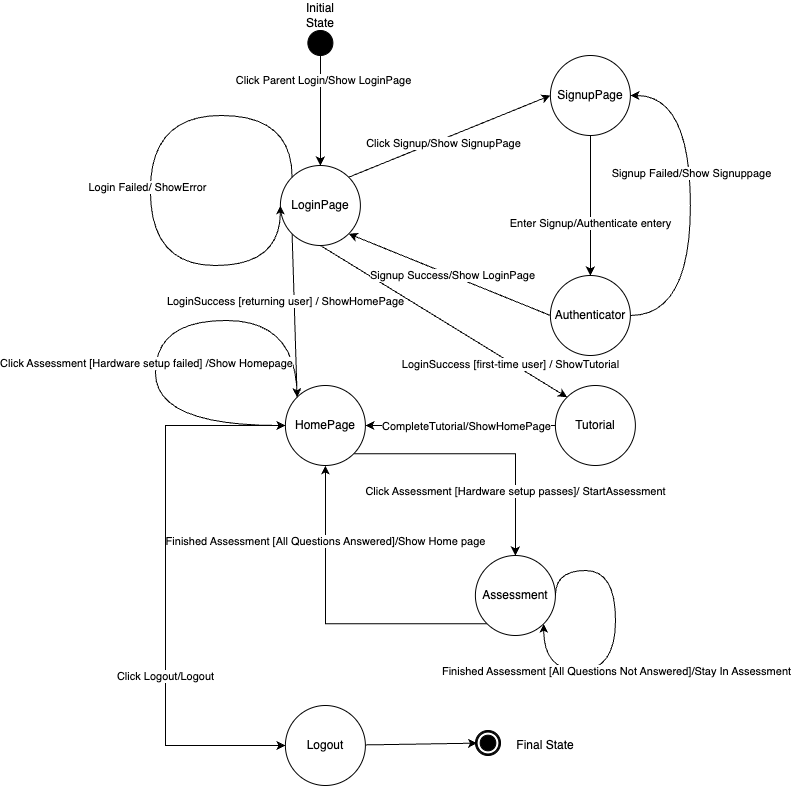
\includegraphics[scale=0.5]{images/TeleHealth_StateMachine.png}
  \caption{Finite State Machine that represents the Parent-Child interaction with the Assessmenet Interface}
\end{figure}

This is the project's most critical element because the system's primary objective is to support parents when conducting at home speech assessments for their child. 
The success of the system is dependent on the parent-child correctly using the interface.
\section{Look and Feel Requirements}
\subsection{Appearance Requirements}
\begin{enumerate}[{LF-AR}1. ]
  \item The platform should maintain a modern, organized, and visually appealing design that looks clean and professional, while not 
  overwhelming users with unnecessary clutter.\\
  \textbf{Rationale: }A clean layout reduces cognitive load, making it easier for users to use the platform effectively without distractions.\\
  \textbf{Fit criterion: }The user interface must return minimal reports of visual confusion or overwhelming elements in usability testing.  
\end{enumerate}
\begin{enumerate}[{LF-AR}2. ]
  \item The platform’s navigation should be intuitive and allow users to quickly understand how to move between different sections.\\
  \textbf{Rationale: }Simple, user-friendly navigation ensures that users can move through the system without confusion, especially since the platform will be used by both children and adults.\\
  \textbf{Fit criterion: }During user testing, at least 95\% of participants must successfully complete navigation-related tasks without external guidance.  
\end{enumerate}
\begin{enumerate}[{LF-AR}3. ]
  \item The design should promote a calm and reassuring environment that is visually appealing but not overstimulating.\\
  \textbf{Rationale: }Children undergoing assessments may feel anxious; a calming design helps create a more comfortable and welcoming environment.\\
  \textbf{Fit criterion: }Feedback from child users and caregivers during usability testing must indicate that the design fosters a calm and positive experience.  
\end{enumerate}
\begin{enumerate}[{LF-AR}4. ]
  \item The assessment interface should be designed to be easily understood by children, with accessible and age-appropriate elements.\\
  \textbf{Rationale: }A simple design tailored to children’s comprehension levels ensures they can participate in the assessment without confusion or frustration.\\
  \textbf{Fit criterion: }In user testing, 95\% of children aged 6-12 must be able to complete a sample assessment without adult assistance.  
\end{enumerate}
\begin{enumerate}[{LF-AR}5. ]
  \item The platform should provide immediate feedback for user interactions, confirming that inputs have been registered.\\
  \textbf{Rationale: }Feedback is important to confirm that the system is responding to user inputs, which is especially critical for children who may be unsure if their actions have been registered.\\
  \textbf{Fit criterion: }100\% of user interactions must trigger an appropriate feedback response within 0.5 seconds.  
\end{enumerate}

\subsection{Style Requirements}
\begin{enumerate}[{LF-SR}1. ]
  \item The design should maintain consistency across all pages to create a cohesive user experience.\\
  \textbf{Rationale: }Consistency in design elements helps reduce user confusion, making the platform easier to navigate and more aesthetically pleasing.\\
  \textbf{Fit criterion: }All visual elements must adhere to a style guide, ensuring a consistent look across 100\% of the platform’s pages.  
\end{enumerate}
\begin{enumerate}[{LF-SR}2. ]
  \item The design should align with the client's established company brand guidelines, including the use of specific colors, logos, or fonts.\\
  \textbf{Rationale: }Aligning with brand guidelines ensures that the platform reflects the client's professional image and maintains brand integrity.\\
  \textbf{Fit criterion: }100\% of the platform’s design elements must comply with the client’s branding guidelines.  
\end{enumerate}

\section{Usability and Humanity Requirements}
\subsection{Ease of Use Requirements} 
\begin{enumerate}[{UH-EOU}1. ]
  \item The system shall be intuitive for new users to understand.\\
  \textbf{Rationale: }New users should not be overwhelmed with the system. New users must be able to understand the system to effectively perform the assessment (parents and children), or view the results (clinicians).\\
  \textbf{Fit criterion: }The duration between starting the assessment to finishing the first question is less than 2 minutes.
  \item The system shall provide detailed instructions on how to use key features of the application, along with its purpose.\\
  \textbf{Rationale: }The system will provide relevant important information about the assessment so the user is informed about the system's usage.\\ 
  \textbf{Fit criterion: }The system will direct the user to additional information prior to starting the setup process, and upon completion of the assessment.
\end{enumerate}
\subsection{Personalization and Internationalization Requirements}
\begin{enumerate}[{UH-PI}1. ]
  \item The system shall support multiple languages.\\
  \textbf{Rationale: }The assessment must be conducted in two languages for the purpose of the research study. As well, it would be beneficial for parents and children to navigate the system in their preferred language.\\
  \textbf{Fit criterion: }The assessment will always be available to be conducted in two different languages (within a single assessment).
\end{enumerate}
\subsection{Learning Requirements}
\begin{enumerate}[{UH-LI}1. ]
  \item The system shall not require additional resources to be navigated.\\
  \textbf{Rationale: }The system should be intuitive to navigate without additional information to simplify the assessment process.\\
  \textbf{Fit criterion: }All information required for the assessment will be directly displayed by the system.
  \item The system shall include a user-guide for additional usage information.\\
  \textbf{Rationale: }User documentation can be helpful for troubleshooting and maintenance should problems arise. This document is optional and not required reading for the user's interactions with the system.\\
  \textbf{Fit criterion: }User documentation will be provided on the team's GitHub upon project completion.
\end{enumerate}
\subsection{Understandability and Politeness Requirements}
\begin{enumerate}[{UH-UP}1. ]
  \item The system will not use technical language when displaying information to the user.\\
  \textbf{Rationale: }The system will be designed for parents and children to participate in assessments, thus the system should make information easily understandable.\\
  As well, clinicians may not have a technological background, so any technical aspects should be communicated in easy to understand terms.\\
  \textbf{Fit criterion: }The system will be reviewed by the team's supervisor and their collaborator to verify all language used is appropriate for users.
\end{enumerate}
\subsection{Accessibility Requirements}
\begin{enumerate}[{UH-AR}1. ]
  \item The system shall be simple and intuitive for assessment interactions with children.\\
  \textbf{Rationale: }Children interacting with the assessment can vary in age and cognitive abilities. To get reliable assessment results, the children participating must understand the system they interact with.\\
  \textbf{Fit criterion: }The assessment will feature minimal display elements, with clear indication of interactions.
\end{enumerate}

\section{Performance Requirements}
\subsection{Speed and Latency Requirements}
\begin{enumerate}[{PR-SL}1. ]
  \item The system shall load web pages within 3 seconds of navigating to it.\\
  \textbf{Rationale: }Fast page loading is critical for maintaining user engagement and reducing user frustrations during the assessment process.\\
  \textbf{Fit criterion: }The web pages must completely be loaded with all functionalities within the 3 seconds of navigation on a standard broadband internet connection.  
\end{enumerate}
\begin{enumerate}[{PR-SL}2. ]
  \item The system must maintain video and audio recording latency of less than 1 second to support accurate data capture for speech assessment.\\
  \textbf{Rationale: }Having high latency could lead to desynchronization between audio and video, causing errors in the timestamps or making it difficult for speech-language pathologists (SLPs) to analyze the recordings properly.\\
  \textbf{Fit criterion: }The difference between a user's actions and the corresponding recording playback should not exceed 1 second.  
\end{enumerate}
\begin{enumerate}[{PR-SL}3. ]
  \item The system must ensure that all video recordings are capture and stored in a resolution of at least 720p.\\
  \textbf{Rationale: }A minimum resolution of 720p is necessary to ensure the video can be accurately processed through visual analysis tools. Lower resolutions may not capture sufficient detail, potentially leading to skewed data and inaccurate assessments for clinicians.\\
  \textbf{Fit criterion: }All video's captured and processed must have a minimum resusoltion of 720p.
\end{enumerate}
\begin{enumerate}[{PR-SL}4. ]
  \item The system must process the data from a session and generate a report within 10 seconds, ensuring quick feedback to users (this requirement is satisfied when FR-DPD2 is fulfilled).\\
  \textbf{Rationale: }Generating the assessment reports for clinicians under 10 seconds is essential for maintaining a smooth workflow. Long delays in report generation could cause unnecessary waiting times and reduce the system's perceived efficiency and user engagement.\\
  \textbf{Fit criterion: }Upon request by clinician, the system must generate a comprehensive report of a the sessions requested within 10 seconds  
\end{enumerate}

\subsection{Safety-Critical Requirements}
\begin{enumerate}[{PR-SCL}1. ]
  \item There are no safety-critical requirements
\end{enumerate}

\subsection{Precision or Accuracy Requirements}
\begin{enumerate}[{PR-PA}1. ]
  \item The system must achieve a audio analysis accuracy of at least 95\% to ensure reliable assessment results for clinicians.\\
  \textbf{Rationale: }It is imporant that the audio analysis accuracy has a high percision rate. Without this level of percision, clinicians could 
  be mislead by inaccurate results affecting the quality of diagnosis and subsequent treatment.\\
  \textbf{Fit criterion: }The speech analysis results will consistently reflect a minimum accuracy rate of 95\%.  
\end{enumerate}
\begin{enumerate}[{PR-PA}2. ]
  \item The system must detect video disturbances with an accuracy of at least 90\% to minimize the impact of visual issues on the assessment data.\\
  \textbf{Rationale: }Detecting video disturbances with 90\% accuracy ensures that visual data remains reliable and helps clinicians get accurate data.\\
  \textbf{Fit criterion: }The system will report video disturbance detection rates that meet or exceed 90\%.  
\end{enumerate}
\begin{enumerate}[{PR-PA}3. ]
  \item The system must ensure that timestamp accuracy is within 1 second to align recorded events with real-time actions for precise analysis.\\
  \textbf{Rationale: }Timestamp accuracy within 1 second ensures that all speech and video events are synchronized precisely, which is essential for accurate analysis of the timing and sequence of interactions. A larger discrepancy could result in data misalignment, skewing the overall assessment and potentially missing critical events.\\
  \textbf{Fit criterion: }Timestamps recorded during assessments will consistently align within a 1-second window, verifying that all events are accurately synchronized.  
\end{enumerate}
\begin{enumerate}[{PR-PA}4. ]
  \item The system must guarantee 100\% accuracy in the assessment answer key to ensure correct evaluation of responses provided by users.\\
  \textbf{Rationale: }Any errors in the answer key could lead to misinterpretation of a child’s abilities or progress, undermining the purpose of the assessment.\\
  \textbf{Fit criterion: }The assessment answer key will be manually be verified to ensure that ti contatins no inaccuracies, ensuring complete correctness of answers.  
\end{enumerate}
\begin{enumerate}[{PR-PA}5. ]
  \item The system must ensure that all questions are 100\% relevant to the purpose of the platform to maintain focus on accurate speech and language assessment.\\
  \textbf{Rationale: }Ensuring that all questions are fully relevant to the platform’s purpose guarantees that the assessment focuses only on aspects critical to speech and language development. Irrelevant questions could confuse users and divert attention from important areas.\\
  \textbf{Fit criterion: }All assessment questions will be manual reviewed to confirm that they align perfectly with the platform's objectives.  
\end{enumerate}

\subsection{Robustness or Fault-Tolerance Requirements}
\begin{enumerate}[{PR-RFT}1. ]
  \item The system must manage any technical errors effectively and provide clear feedback to users when issues occur.\\
  \textbf{Rationale: }Proper error handling prevents user confusion and improves the user experience. Without it, users may not understand if something is wrong or why the system is not working as they expect, leading to frustration.\\
  \textbf{Fit criterion: }The system must display error messages for at least 95\% of common user errors.  
\end{enumerate}
\begin{enumerate}[{PR-RFT}2. ]
  \item The system must implement data backup and recovery processes to protect user data and assessment results.\\
  \textbf{Rationale: }Effective backup and recovery ensure that user data is not lost during a system failure. Data loss could disrupt assessments and treatment plans.\\
  \textbf{Fit criterion: }The system must back up data on the first of every month within a 4hr timeframe.  
\end{enumerate}
\begin{enumerate}[{PR-RFT}3. ]
  \item The system must validate inputs to accept only specified formats during user interactions.\\
  \textbf{Rationale: }Strict input validation prevents errors and enhances data integrity. It also protects the system from malicious inputs that could cause issues.\\
  \textbf{Fit criterion: }The system must reject 100\% of invalid inputs and display appropriate error messages to users.  
\end{enumerate}

\subsection{Capacity Requirements}
\begin{enumerate}[{PR-CR}1. ]
  \item The system must accommodate a minimum of 2000 user accounts at launch.\\
  \textbf{Rationale: }Supporting at least 2000 user accounts ensures the system meets initial demand and allows for growth in user adoption.\\
  \textbf{Fit criterion: }The system must successfully manage 2000 user accounts at deployment without stability issues.  
\end{enumerate}
\begin{enumerate}[{PR-CR}2. ]
  \item The system must have the capacity to store a minimum of 10TB of data each year.\\
  \textbf{Rationale: }Storing 10TB of data annually ensures that all user data and assessment results are preserved and accessible for analysis and reporting. This capacity is essential for maintaining comprehensive records over time.\\
  \textbf{Fit criterion: }The database must have 10TB of allocated space at the start of every year.  
\end{enumerate}
\begin{enumerate}[{PR-CR}3. ]
  \item The system must support a minimum of 200 concurrent users simultaneously upon initial release, and have the capability to scale to accommodate more users as demand increases.\\
  \textbf{Rationale: }Supporting 200 concurrent users is necessary to handle peak usage times effectively. The ability to scale ensures that performance remains stable as user demand grows.\\
  \textbf{Fit criterion: }The system must maintain stable performance levels (e.g throughput, error rate) while supporting 200 concurrent users.  
\end{enumerate}
\begin{enumerate}[{PR-CR}4. ]
  \item The system must support a minimum of 100 concurrent video and audio recording uploads simultaneously and have the capability to scale to accommodate more users as demand increases.\\
  \textbf{Rationale: }Supporting 100 concurrent user uploads is necessary to handle peak usage times effectively. The ability to scale ensures that performance remains stable as user demand grows.\\
  \textbf{Fit criterion: }The system must maintain stable performance levels (e.g throughput, error rate) while supporting 100 concurrent uploads.  
\end{enumerate}

\subsection{Scalability or Extensibility Requirements}
\begin{enumerate}[{PR-SE}1. ]
  \item The system must support the addition of new user accounts without compromising performance.\\
  \textbf{Rationale: }User scalability is essential to accommodate growth in the user base and ensure consistent performance as more users engage with the platform.\\
  \textbf{Fit criterion: }The system must effectively manage a user base increase of at least 10\% annually while maintaining performance metrics defined in the capacity requirements.  
\end{enumerate}
\begin{enumerate}[{PR-SE}2. ]
  \item The system must handle increasing volumes of data without loss of performance or data integrity.\\
  \textbf{Rationale: }Data scalability ensures that as the volume of stored data grows, the system can still process, retrieve, and manage this data efficiently. This is crucial for maintaining system reliability and providing accurate insights from the collected data.\\
  \textbf{Fit criterion: }The system must manage a data increase of at least 10\% annually.  
\end{enumerate}
\begin{enumerate}[{PR-SE}3. ]
  \item The system must expand processing capabilities to handle increased computational demands.\\
  \textbf{Rationale: }Processing scalability is vital for ensuring that the system can efficiently perform analyses and computations as the number of users or the complexity of tasks increases. This prevents bottlenecks in data processing and ensures timely results for clinicians.\\
  \textbf{Fit criterion: }The system must increase data processing capacity by at least 2\% without impacting response times for data processing tasks.  
\end{enumerate}

\subsection{Longevity Requirements}
\begin{enumerate}[{PR-LR}1. ]
  \item The system must function reliably without significant malfunctions in the release build, even as further development and updates are implemented.\\
  \textbf{Rationale: }Ensuring stability during ongoing development is crucial to maintain user trust and provide uninterrupted service. Any major malfunctions could lead to user frustration and potential loss of users, impacting the system's reputation.\\
  \textbf{Fit criterion: }The system must demonstrate a failure rate of less than 1\% in the release build during ongoing development, ensuring that users experience minimal disruptions.  
\end{enumerate}
\begin{enumerate}[{PR-LR}2. ]
  \item The system must be compatible with major operating systems, including Windows, macOS, Linux, Android, and iOS.\\
  \textbf{Rationale: }Broad compatibility ensures that the system can reach a wider audience, providing access to users regardless of their device or operating system. This is essential for maximizing user engagement and satisfaction.\\
  \textbf{Fit criterion: }The system must pass compatibility tests on all specified operating systems, with successful operation and user experience validated on each platform.  
\end{enumerate}

\section{Operational and Environmental Requirements}
\subsection{Expected Physical Environment}
\begin{enumerate}[{OE-EPE}1. ]
  \item The system can be run on all browser-supported devices regardless of screen sizes.\\
  \textbf{Rationale: }The system will be run on a variety of devices through web browsers, and should adapt the different screen sizes so users get full functionality.\\
  \textbf{Fit criterion: }The system's displayed elements will scale appropriately to different screen sizes.
\end{enumerate}
\subsection{Wider Environment Requirements}
\begin{enumerate}[{OE-WE}1. ]
  \item The system shall be used in a quiet environment.\\
  \textbf{Rationale: }The system will be performing audio and video analysis, and conducting the assessment in a loud or busy environment could lead to unexpected results due to noise.\\
  \textbf{Fit criterion: }The system will inform the user, prior to setup, that the optimal experience for the assessment is in a quiet environment. 
  \item The system shall be used with an internet connection.\\
  \textbf{Rationale: }The assessment will be conducted online, and not saved locally on the user's device. Therefore, an internet connection is required.\\
  \textbf{Fit criterion: }The system will be accessed online. The system will inform the user, prior to setup, that the assessment will be conducted online, and no files will be downloaded to their device for the assessment. 
\end{enumerate}
\subsection{Requirements for Interfacing with Adjacent Systems}
\begin{enumerate}[{OE-IA}1. ]
  \item The system shall be hosted on an external server for retrieving and storing data.\\
  \textbf{Rationale: }The supervisor's collaborator is running the current system on an external server, which the new system will utilize.\\
  \textbf{Fit criterion: }The system (including the assessment) will be published and accessed through the external server.
\end{enumerate}
\subsection{Productization Requirements}
\begin{enumerate}[{OE-PR}1. ]
  \item N/A
\end{enumerate}
\subsection{Release Requirements}
\begin{enumerate}[{OE-RR}1. ]
  \item N/A
\end{enumerate}

\section{Maintainability and Support Requirements}
\subsection{Maintenance Requirements}
\begin{enumerate}[{MS-MR}1. ]
  \item The platform should be built using a modular architecture so that different components may be updated or replaced independently without disrupting the entire system.\\
  \textbf{Rationale: }Modular systems are easier to maintain and update, reducing downtime and ensuring new features or bug fixes can be implemented without impacting the core functionality of the platform.\\
  \textbf{Fit criterion: }Any update of an individual component shall have no more than 10 lines of code edited outside of the component.
\end{enumerate}

\subsection{Supportability Requirements}
\begin{enumerate}[{MS-SR}1. ]
  \item Users should be able to submit feature requests or report issues directly to the platform’s GitHub repository, ensuring that the development team can track and prioritize improvements or bug fixes.\\
  \textbf{Rationale: }Centralizing feature requests and issue tracking in GitHub makes it easier for the development team to manage feedback and streamline future updates.\\
  \textbf{Fit criterion: }The platform must include a direct link to the GitHub repository, with a clear option for users to submit requests or report issues, and GitHub should have dedicated categories for issues, 
  feature requests, and feedback.
\end{enumerate}
\begin{enumerate}[{MS-SR}2. ]
  \item The platform should provide a comprehensive, easy-to-follow tutorial that guides users through the website and the assessment process.\\
  \textbf{Rationale: }Tutorials help users understand the functionality of the platform, reducing the need for external support and improving user experience, particularly for new users or children.\\
  \textbf{Fit criterion: }The tutorial must be accessible from the homepage and should cover all core functionalities. In usability testing, 90\% of users should be able to complete tasks correctly after following the
   tutorial.
\end{enumerate}

\subsection{Adaptability Requirements}
\begin{enumerate}[{MS-AR}1. ]
  \item The platform should be responsive, automatically adjusting its layout and design to suit different screen sizes, including desktops, tablets, and mobile devices.\\
  \textbf{Rationale: }A responsive design ensures the platform is accessible on any device, providing a seamless user experience regardless of screen size or resolution.\\
  \textbf{Fit criterion: }The platform’s interface should render correctly on screens ranging from 4” (mobile) to 27” (desktop) with no loss of functionality or readability. Testing must show that 100\% of essential 
  features are usable on all screen sizes.
\end{enumerate}

\section{Security Requirements}
\subsection{Access Requirements}
\begin{enumerate}[{SR-AC}1. ]
  \item Only users with an Admin role can create and assign accounts to clinicians.\\
  \textbf{Rationale: }Full access of the system and permissions including creating clinician accounts should only be available to admin roles by the system. \\
  \textbf{Fit criterion: }Admin users will have full access to the system including create clinician accounts, viewing data records, and starting assessments. 
  \item Users with parent roles can complete assessments.\\
  \textbf{Rationale: }Users with a parent role should have the ability to create accounts and complete assessments with their children on the system.\\
  \textbf{Fit criterion: }Users with parent roles will only be able to create a parent account, login to the system, have access to completing the assessments, and logging off the system 
  \item Users with clinician roles can view assessment results.\\
  \textbf{Rationale: }Clinicians must be able to see all video and audio recordings of completed assessments, as well as the analyzed results from the system to aid in their research. \\
  \textbf{Fit criterion: }User with a clinician role will not be able to log in to a parent account and start/complete assessments. 
  \item Users shall input their username and password to securely login.\\
  \textbf{Rationale: }Users should be able to securely login by inputting their login credentials to ensure to prevent unauthorized access. \\
  \textbf{Fit criterion: }A user should not be able to login to an account they do not have the required credentials for.
\end{enumerate}
\subsection{Integrity Requirements}
\begin{enumerate}[{SR-INT}1. ]
  \item N/A
\end{enumerate}
\subsection{Privacy Requirements}
\begin{enumerate}[{SR-P}1. ]
  \item The system shall adhere to all data protection and privacy laws in the region its used.\\
  \textbf{Rationale: }The system will respect the privacy and confidentiality of all users to adhere to all applicable protection laws.\\
  \textbf{Fit criterion: }The system will be reviewed prior to public release to ensure it follows all applicable protection laws
  \item The system shall encrypt all sensitive data in transit and at rest to keep data confidential.\\
  \textbf{Rationale: }The system should encrypt sensitive data at all times to ensure high level of security to protect user information from potential data footage leaks, and unauthorized access \\
  \textbf{Fit criterion: }Data follows the standard encryption protocol at all times; data is encrypted when in transit and only decrypted when viewed by clinician user for analysis purposes.
  \item The system shall not collect any personal identifiable information from the user.\\
  \textbf{Rationale: }The system should not collect any personal identifiable information to ensure confidentially of all video and audio recordings associated with the user. \\
  \textbf{Fit criterion: }The system does not store any personal identifiable information. All data stored includes, username, and data/audio recordings only. 
\end{enumerate}
\subsection{Audit Requirements}
\begin{enumerate}[{SR-AU}1. ]
  \item N/A
\end{enumerate}
\subsection{Immunity Requirements}
\begin{enumerate}[{SR-IM}1. ]
  \item The system must mandate strong passwords.\\
  \textbf{Rationale: }The system must require a strong password mandate to secure user accounts from unauthorized access.\\
  \textbf{Fit criterion: }The system will complete account creation upon entering a valid password that follows the specified mandate. 
\end{enumerate}

\section{Cultural Requirements}
\subsection{Cultural Requirements}
\begin{enumerate}[{CU-CR}1. ]
  \item The platform must not contain any language or imagery that could be considered culturally insensitive or offensive to any users, particularly the primary user groups.\\
  \textbf{Rationale: }Ensuring cultural sensitivity is critical in a healthcare setting, especially when working with diverse populations. Avoiding insensitive content fosters a respectful and inclusive environment 
  for users.\\
  \textbf{Fit criterion: }During user acceptance testing and content review, 100\% of language and imagery used on the platform must be validated by at least 5 representatives of the primary user groups to ensure no instances of 
  insensitivity.
\end{enumerate}
\begin{enumerate}[{CU-CR}2. ]
  \item The platform should be bilingual, supporting both English and Mandarin for all user interfaces and assessments to accommodate the language preferences of users.\\
  \textbf{Rationale: }Given that the target user base includes bilingual children, providing language options ensures accessibility and inclusivity, allowing users to complete assessments in their choice of language.\\
  \textbf{Fit criterion: }100\% of text, instructions, and assessments must be fully translated and accessible in both English and Mandarin, with no language discrepancies or untranslated segments.  
\end{enumerate}

\section{Compliance Requirements}
\subsection{Legal Requirements}
\begin{enumerate}[{CR-LR}1. ]
  \item N/A
\end{enumerate}
\subsection{Standards Compliance Requirements}
\begin{enumerate}[{CR-STD}1. ]
  \item The system shall use security measures to protect all stored user assessment data.\\
  \textbf{Rationale: }The system must use strong security measures to protect sensitive and confidential user information including collected video and audio recordings from assessment results to ensure privacy and integrity.\\
  \textbf{Fit criterion: }All stored user assessment data is only associated with a username. 

\end{enumerate}

\section*{Traceability Matrix}
\begin{table}[!ht]
  \centering
  \resizebox{\textwidth}{!}{
  \begin{tabular}{|l|l|l|l|l|l|l|l|l|l|l|l|l|l|l|l|l|l|l|l|l|l|l|l|l|l|l|l|l|l|l|l|}
  \hline
      PUC no & 1 & 2 & 3 & 4 & 5 & 6 & 7 & 8 & 9 & 10 & 11 & 12 & 13 & 14 & 15 & 16 & 17 & 18 & 19 & 20 & 21 & 22 & 23 & 24 & 25 & 26 & 27 & 28 & 29 & 30 & 31 \\ \hline
      FR-A1 & ~ & ~ & ~ & X & X & ~ & ~ & ~ & ~ & ~ & ~ & ~ & ~ & ~ & ~ & ~ & ~ & ~ & ~ & ~ & ~ & ~ & ~ & ~ & ~ & ~ & ~ & ~ & ~ & ~ & ~ \\ \hline
      FR-A2 & X & X & ~ & ~ & ~ & ~ & ~ & ~ & ~ & ~ & ~ & ~ & ~ & ~ & ~ & ~ & ~ & ~ & ~ & ~ & ~ & ~ & ~ & ~ & ~ & ~ & ~ & ~ & ~ & ~ & ~ \\ \hline
      FR-A3 & ~ & X & X & ~ & ~ & ~ & ~ & ~ & ~ & ~ & ~ & ~ & ~ & ~ & ~ & ~ & ~ & ~ & ~ & ~ & ~ & ~ & ~ & ~ & ~ & ~ & ~ & ~ & ~ & ~ & ~ \\ \hline
      FR-A4 & ~ & ~ & ~ & X & ~ & X & X & X & ~ & ~ & ~ & ~ & ~ & ~ & ~ & ~ & ~ & ~ & ~ & ~ & ~ & ~ & ~ & ~ & ~ & ~ & ~ & ~ & ~ & ~ & ~ \\ \hline
      FR-A5 & ~ & ~ & ~ & X & ~ & ~ & ~ & ~ & ~ & ~ & ~ & ~ & ~ & ~ & ~ & ~ & ~ & ~ & ~ & ~ & ~ & ~ & ~ & ~ & ~ & ~ & ~ & ~ & ~ & ~ & ~ \\ \hline
      FR-SS1 & ~ & ~ & ~ & ~ & ~ & ~ & ~ & ~ & X & ~ & ~ & ~ & ~ & X & ~ & ~ & ~ & ~ & ~ & ~ & ~ & ~ & ~ & ~ & ~ & ~ & ~ & ~ & ~ & ~ & ~ \\ \hline
      FR-SS2 & ~ & ~ & ~ & ~ & ~ & ~ & ~ & ~ & ~ & ~ & X & ~ & ~ & ~ & ~ & ~ & ~ & ~ & ~ & ~ & ~ & ~ & ~ & ~ & ~ & ~ & ~ & ~ & ~ & ~ & ~ \\ \hline
      FR-SS3 & ~ & ~ & ~ & ~ & ~ & ~ & ~ & ~ & ~ & ~ & X & ~ & ~ & ~ & ~ & ~ & ~ & ~ & ~ & ~ & ~ & ~ & ~ & ~ & ~ & ~ & ~ & ~ & ~ & ~ & ~ \\ \hline
      FR-SS4 & ~ & ~ & ~ & ~ & ~ & ~ & ~ & ~ & ~ & ~ & ~ & ~ & ~ & X & ~ & ~ & ~ & ~ & ~ & ~ & ~ & ~ & ~ & ~ & ~ & ~ & ~ & ~ & ~ & ~ & ~ \\ \hline
      FR-SS5 & ~ & ~ & ~ & ~ & ~ & ~ & ~ & ~ & ~ & ~ & ~ & ~ & ~ & ~ & X & ~ & ~ & ~ & ~ & ~ & ~ & ~ & ~ & ~ & ~ & ~ & ~ & ~ & ~ & ~ & ~ \\ \hline
      FR-AI1 & ~ & ~ & ~ & ~ & ~ & ~ & ~ & ~ & ~ & ~ & ~ & ~ & X & ~ & X & ~ & ~ & ~ & ~ & ~ & ~ & ~ & ~ & ~ & ~ & ~ & ~ & ~ & ~ & ~ & ~ \\ \hline
      FR-AI2 & ~ & ~ & ~ & ~ & ~ & ~ & ~ & ~ & ~ & ~ & ~ & ~ & ~ & ~ & ~ & ~ & ~ & X & ~ & ~ & ~ & ~ & ~ & ~ & ~ & ~ & ~ & ~ & ~ & ~ & ~ \\ \hline
      FR-AI3 & ~ & ~ & ~ & ~ & ~ & ~ & ~ & ~ & ~ & ~ & ~ & ~ & ~ & ~ & ~ & ~ & X & ~ & ~ & ~ & ~ & ~ & ~ & ~ & ~ & ~ & ~ & ~ & ~ & ~ & ~ \\ \hline
      FR-AI4 & ~ & ~ & ~ & ~ & ~ & ~ & ~ & ~ & ~ & ~ & ~ & ~ & ~ & ~ & ~ & ~ & X & ~ & X & ~ & ~ & ~ & ~ & ~ & ~ & ~ & ~ & ~ & ~ & ~ & ~ \\ \hline
      FR-AI5 & ~ & ~ & ~ & ~ & ~ & ~ & ~ & ~ & ~ & ~ & ~ & ~ & ~ & ~ & ~ & ~ & ~ & ~ & ~ & X & ~ & ~ & ~ & ~ & ~ & ~ & ~ & ~ & ~ & ~ & ~ \\ \hline
      FR-AI6 & ~ & ~ & ~ & ~ & ~ & ~ & ~ & ~ & ~ & ~ & ~ & ~ & ~ & ~ & ~ & X & ~ & ~ & ~ & ~ & ~ & ~ & ~ & ~ & ~ & ~ & ~ & ~ & ~ & ~ & ~ \\ \hline
      FR-AI7 & ~ & ~ & ~ & ~ & ~ & ~ & ~ & ~ & ~ & ~ & ~ & ~ & ~ & ~ & ~ & ~ & ~ & ~ & ~ & ~ & X & ~ & ~ & ~ & ~ & ~ & ~ & ~ & ~ & ~ & ~ \\ \hline
      FR-DSC1 & ~ & ~ & ~ & ~ & ~ & ~ & ~ & ~ & ~ & ~ & ~ & X & ~ & ~ & ~ & ~ & ~ & ~ & ~ & ~ & ~ & ~ & ~ & ~ & ~ & ~ & ~ & ~ & ~ & ~ & ~ \\ \hline
      FR-DSC2 & ~ & ~ & ~ & ~ & ~ & ~ & ~ & ~ & ~ & ~ & ~ & X & ~ & ~ & ~ & ~ & ~ & ~ & ~ & ~ & ~ & ~ & ~ & ~ & ~ & ~ & X & X & X & ~ & ~ \\ \hline
      FR-DSC3 & ~ & ~ & ~ & ~ & ~ & ~ & ~ & ~ & ~ & ~ & ~ & X & ~ & ~ & ~ & ~ & ~ & ~ & ~ & ~ & ~ & ~ & ~ & ~ & ~ & ~ & ~ & ~ & ~ & ~ & ~ \\ \hline
      FR-DSC4 & ~ & ~ & ~ & ~ & ~ & ~ & ~ & ~ & ~ & ~ & ~ & X & ~ & ~ & ~ & ~ & ~ & ~ & ~ & ~ & ~ & X & ~ & ~ & ~ & ~ & ~ & ~ & ~ & ~ & ~ \\ \hline
      FR-DSC5 & ~ & ~ & ~ & ~ & ~ & ~ & ~ & ~ & ~ & ~ & ~ & ~ & ~ & ~ & ~ & ~ & ~ & ~ & ~ & ~ & ~ & ~ & ~ & ~ & ~ & ~ & ~ & ~ & ~ & ~ & X \\ \hline
      FR-VADA1 & ~ & ~ & ~ & ~ & ~ & ~ & ~ & ~ & ~ & ~ & ~ & X & ~ & ~ & ~ & ~ & ~ & ~ & ~ & ~ & ~ & ~ & ~ & ~ & ~ & ~ & ~ & ~ & ~ & ~ & ~ \\ \hline
      FR-VADA2 & ~ & ~ & ~ & ~ & ~ & ~ & ~ & ~ & ~ & ~ & ~ & ~ & ~ & ~ & ~ & ~ & ~ & ~ & ~ & ~ & ~ & ~ & X & X & X & X & ~ & ~ & ~ & ~ & ~ \\ \hline
      FR-VADA3 & ~ & ~ & ~ & ~ & ~ & ~ & ~ & ~ & ~ & ~ & ~ & ~ & ~ & ~ & ~ & ~ & ~ & ~ & ~ & ~ & ~ & ~ & ~ & ~ & ~ & ~ & X & X & X & ~ & ~ \\ \hline
      FR-DPD1 & ~ & ~ & ~ & ~ & ~ & ~ & ~ & ~ & ~ & ~ & ~ & ~ & ~ & ~ & ~ & ~ & ~ & ~ & ~ & ~ & ~ & ~ & ~ & ~ & ~ & ~ & X & X & ~ & ~ & ~ \\ \hline
      FR-DPD2 & ~ & ~ & ~ & ~ & ~ & ~ & ~ & ~ & ~ & ~ & ~ & ~ & ~ & ~ & ~ & ~ & ~ & ~ & ~ & ~ & ~ & ~ & ~ & ~ & ~ & ~ & ~ & ~ & ~ & X & ~ \\ \hline
      FR-DPD3 & ~ & ~ & ~ & ~ & ~ & ~ & ~ & ~ & ~ & ~ & ~ & ~ & ~ & ~ & ~ & ~ & ~ & ~ & ~ & ~ & ~ & ~ & ~ & ~ & ~ & ~ & ~ & ~ & ~ & X & ~ \\ \hline
      FR-DPD4 & ~ & ~ & ~ & ~ & ~ & ~ & ~ & ~ & ~ & X & ~ & ~ & ~ & ~ & ~ & ~ & ~ & ~ & ~ & ~ & ~ & ~ & ~ & ~ & ~ & ~ & ~ & ~ & ~ & ~ & ~ \\ \hline
  \end{tabular}}
  \caption{Traceability Matrix for PUCs and FRs}
\end{table}

\begin{table}[!ht]
  \centering
  \resizebox{\textwidth}{!}{
  \begin{tabular}{|l|l|l|l|l|l|l|l|l|l|l|l|l|l|l|l|l|l|l|l|l|l|l|l|l|l|l|l|l|l|l|l|}
  \hline
      PUC no & 1 & 2 & 3 & 4 & 5 & 6 & 7 & 8 & 9 & 10 & 11 & 12 & 13 & 14 & 15 & 16 & 17 & 18 & 19 & 20 & 21 & 22 & 23 & 24 & 25 & 26 & 27 & 28 & 29 & 30 & 31 \\ \hline
      LF-AR1 & X & ~ & X & X & X & X & X & X & X & X & X & ~ & ~ & X & X & ~ & X & X & X & X & X & ~ & ~ & ~ & ~ & ~ & ~ & ~ & ~ & X & ~ \\ \hline
      LF-AR2 & X & ~ & X & X & X & ~ & ~ & ~ & X & X & X & ~ & ~ & X & X & ~ & ~ & ~ & ~ & ~ & X & ~ & ~ & ~ & ~ & ~ & ~ & ~ & ~ & X & ~ \\ \hline
      LF-AR3 & ~ & ~ & ~ & ~ & ~ & ~ & ~ & ~ & X & ~ & X & ~ & ~ & X & X & ~ & X & X & X & X & X & ~ & ~ & ~ & ~ & ~ & ~ & ~ & ~ & ~ & ~ \\ \hline
      LF-AR4 & ~ & ~ & ~ & ~ & ~ & ~ & ~ & ~ & X & ~ & X & ~ & ~ & X & X & ~ & X & X & X & X & X & ~ & ~ & ~ & ~ & ~ & ~ & ~ & ~ & ~ & ~ \\ \hline
      LF-AR5 & X & X & X & X & X & X & X & X & ~ & ~ & X & ~ & X & ~ & X & X & ~ & X & X & X & X & ~ & ~ & ~ & ~ & ~ & ~ & ~ & ~ & X & ~ \\ \hline
      LF-SR1 & ~ & ~ & ~ & ~ & ~ & ~ & ~ & ~ & X & X & ~ & ~ & ~ & ~ & X & ~ & X & ~ & X & ~ & X & ~ & ~ & ~ & ~ & ~ & ~ & ~ & ~ & X & ~ \\ \hline
      LF-SR2 & ~ & ~ & ~ & ~ & ~ & ~ & ~ & ~ & X & ~ & ~ & ~ & ~ & X & ~ & ~ & X & ~ & ~ & ~ & X & ~ & ~ & ~ & ~ & ~ & ~ & ~ & ~ & X & ~ \\ \hline
      UH-EOU1 & X & ~ & X & X & X & ~ & ~ & ~ & X & X & X & ~ & X & X & X & ~ & X & X & X & X & X & ~ & ~ & ~ & ~ & ~ & ~ & ~ & ~ & X & ~ \\ \hline
      UH-EOU2 & X & X & X & ~ & X & ~ & ~ & ~ & X & X & X & ~ & ~ & X & ~ & ~ & ~ & ~ & ~ & ~ & ~ & ~ & ~ & ~ & ~ & ~ & ~ & ~ & ~ & ~ & ~ \\ \hline
      UH-PI1 & ~ & ~ & ~ & ~ & ~ & ~ & ~ & ~ & X & ~ & X & ~ & ~ & X & X & ~ & X & X & ~ & ~ & X & ~ & ~ & ~ & ~ & ~ & ~ & ~ & ~ & X & ~ \\ \hline
      UH-LI1 & ~ & ~ & ~ & ~ & ~ & ~ & ~ & ~ & X & X & X & ~ & X & X & ~ & ~ & ~ & ~ & ~ & ~ & ~ & ~ & ~ & ~ & ~ & ~ & ~ & ~ & ~ & X & ~ \\ \hline
      UH-LI2 & ~ & ~ & ~ & ~ & ~ & ~ & ~ & ~ & X & ~ & ~ & ~ & ~ & X & ~ & ~ & ~ & ~ & ~ & ~ & ~ & ~ & ~ & ~ & ~ & ~ & ~ & ~ & ~ & ~ & ~ \\ \hline
      UH-UP1 & X & X & ~ & X & X & ~ & ~ & ~ & X & ~ & X & ~ & ~ & X & X & ~ & X & X & X & X & X & ~ & ~ & ~ & ~ & ~ & ~ & ~ & ~ & ~ & ~ \\ \hline
      UH-AR1 & ~ & ~ & ~ & ~ & ~ & ~ & ~ & ~ & X & ~ & X & ~ & ~ & X & X & ~ & X & X & X & X & X & ~ & ~ & ~ & ~ & ~ & ~ & ~ & ~ & ~ & ~ \\ \hline
      PR-SL1 & X & ~ & X & X & ~ & ~ & X & ~ & X & X & X & ~ & ~ & X & X & ~ & X & ~ & ~ & ~ & X & ~ & ~ & ~ & ~ & ~ & ~ & ~ & ~ & X & ~ \\ \hline
      PR-SL2 & ~ & ~ & ~ & ~ & ~ & ~ & ~ & ~ & ~ & ~ & ~ & ~ & X & ~ & ~ & ~ & ~ & ~ & ~ & ~ & ~ & ~ & X & X & X & X & ~ & ~ & ~ & ~ & ~ \\ \hline
      PR-SL3 & ~ & ~ & ~ & ~ & ~ & ~ & ~ & ~ & ~ & ~ & ~ & X & ~ & ~ & ~ & ~ & ~ & ~ & ~ & ~ & ~ & ~ & ~ & ~ & X & X & ~ & ~ & ~ & ~ & ~ \\ \hline
      PR-SL4 & ~ & ~ & ~ & ~ & ~ & ~ & ~ & ~ & ~ & ~ & ~ & ~ & ~ & ~ & ~ & ~ & ~ & ~ & ~ & ~ & ~ & ~ & X & X & X & X & X & X & X & X & ~ \\ \hline
      PR-PA1 & ~ & ~ & ~ & ~ & ~ & ~ & ~ & ~ & ~ & ~ & ~ & ~ & ~ & ~ & ~ & ~ & ~ & ~ & ~ & ~ & ~ & ~ & X & X & ~ & ~ & X & ~ & ~ & ~ & ~ \\ \hline
      PR-PA2 & ~ & ~ & ~ & ~ & ~ & ~ & ~ & ~ & ~ & ~ & ~ & ~ & ~ & ~ & ~ & ~ & ~ & ~ & ~ & ~ & ~ & ~ & ~ & ~ & X & X & X & ~ & ~ & ~ & ~ \\ \hline
      PR-PA3 & ~ & ~ & ~ & ~ & ~ & ~ & ~ & ~ & ~ & ~ & ~ & ~ & ~ & ~ & ~ & ~ & ~ & ~ & ~ & ~ & ~ & ~ & ~ & ~ & ~ & ~ & ~ & X & ~ & ~ & ~ \\ \hline
      PR-PA4 & ~ & ~ & ~ & ~ & ~ & ~ & ~ & ~ & ~ & ~ & ~ & ~ & ~ & ~ & ~ & ~ & ~ & ~ & ~ & ~ & ~ & X & ~ & ~ & ~ & ~ & ~ & ~ & ~ & X & ~ \\ \hline
      PR-PA5 & ~ & ~ & ~ & ~ & ~ & ~ & ~ & ~ & ~ & ~ & ~ & ~ & ~ & ~ & ~ & ~ & X & ~ & ~ & ~ & ~ & ~ & ~ & ~ & ~ & ~ & ~ & ~ & ~ & ~ & ~ \\ \hline
      PR-RFT1 & X & X & X & X & X & X & X & ~ & X & X & X & ~ & X & X & X & X & X & X & ~ & X & X & ~ & ~ & ~ & ~ & ~ & ~ & ~ & ~ & X & ~ \\ \hline
      PR-RFT2 & X & ~ & X & ~ & ~ & ~ & ~ & ~ & ~ & ~ & ~ & X & ~ & ~ & ~ & X & ~ & ~ & ~ & ~ & ~ & X & ~ & ~ & ~ & ~ & ~ & ~ & X & ~ & X \\ \hline
      PR-RFT3 & X & X & X & X & X & ~ & ~ & ~ & ~ & ~ & X & ~ & ~ & ~ & ~ & ~ & ~ & ~ & X & X & ~ & ~ & ~ & ~ & ~ & ~ & ~ & ~ & ~ & ~ & ~ \\ \hline
      PR-CR1 & X & ~ & X & ~ & ~ & ~ & ~ & ~ & ~ & ~ & ~ & ~ & ~ & ~ & ~ & ~ & ~ & ~ & ~ & ~ & ~ & ~ & ~ & ~ & ~ & ~ & ~ & ~ & ~ & ~ & ~ \\ \hline
      PR-CR2 & X & ~ & X & ~ & ~ & ~ & ~ & ~ & ~ & ~ & ~ & X & ~ & ~ & ~ & ~ & ~ & ~ & ~ & ~ & ~ & X & ~ & ~ & ~ & ~ & ~ & ~ & X & ~ & X \\ \hline
      PR-CR3 & ~ & ~ & ~ & X & ~ & ~ & ~ & ~ & ~ & ~ & ~ & ~ & ~ & ~ & X & ~ & ~ & ~ & ~ & ~ & ~ & X & ~ & ~ & ~ & ~ & ~ & ~ & ~ & ~ & ~ \\ \hline
      PR-CR4 & ~ & ~ & ~ & ~ & ~ & ~ & ~ & ~ & ~ & ~ & ~ & ~ & X & ~ & ~ & ~ & ~ & ~ & ~ & ~ & ~ & X & ~ & ~ & ~ & ~ & ~ & ~ & ~ & ~ & ~ \\ \hline
      PR-SE1 & X & X & X & ~ & ~ & ~ & ~ & ~ & ~ & ~ & ~ & ~ & ~ & ~ & ~ & ~ & ~ & ~ & ~ & ~ & ~ & ~ & ~ & ~ & ~ & ~ & ~ & ~ & ~ & ~ & ~ \\ \hline
      PR-SE2 & ~ & ~ & ~ & ~ & ~ & ~ & ~ & ~ & ~ & ~ & ~ & X & ~ & ~ & ~ & ~ & ~ & ~ & ~ & ~ & ~ & X & ~ & ~ & ~ & ~ & ~ & ~ & X & ~ & X \\ \hline
      PR-SE3 & ~ & ~ & ~ & ~ & ~ & ~ & ~ & ~ & ~ & ~ & ~ & ~ & ~ & ~ & ~ & ~ & ~ & ~ & ~ & ~ & ~ & ~ & X & X & X & X & X & X & ~ & ~ & ~ \\ \hline
      PR-LR1 & X & X & X & X & X & X & X & X & X & X & X & X & X & X & X & X & X & X & X & X & X & X & X & X & X & X & X & X & X & X & X \\ \hline
      PR-LR2 & X & X & X & X & X & X & X & X & X & X & X & X & X & X & X & X & X & X & X & X & X & X & X & X & X & X & X & X & X & X & X \\ \hline
      OE-EPE1 & ~ & ~ & ~ & X & ~ & ~ & ~ & ~ & X & X & X & ~ & X & X & X & ~ & X & X & X & X & X & ~ & ~ & ~ & ~ & ~ & ~ & ~ & ~ & X & ~ \\ \hline
      OE-WE1 & ~ & ~ & ~ & ~ & ~ & ~ & ~ & ~ & ~ & ~ & ~ & ~ & X & ~ & ~ & ~ & ~ & ~ & ~ & ~ & ~ & ~ & ~ & ~ & ~ & ~ & ~ & ~ & ~ & ~ & ~ \\ \hline
      OE-WE2 & ~ & ~ & ~ & X & ~ & ~ & ~ & ~ & X & X & ~ & X & ~ & ~ & ~ & ~ & X & ~ & ~ & X & ~ & X & ~ & ~ & ~ & ~ & ~ & ~ & X & X & X \\ \hline
      OE-IA1 & ~ & ~ & ~ & ~ & ~ & ~ & ~ & ~ & ~ & ~ & ~ & X & ~ & ~ & ~ & ~ & ~ & ~ & ~ & ~ & ~ & X & ~ & ~ & ~ & ~ & ~ & ~ & X & ~ & X \\ \hline
      MS-MR1 & X & X & X & X & X & X & X & X & X & X & X & X & X & X & X & X & X & X & X & X & X & X & X & X & X & X & X & X & X & X & X \\ \hline
      MS-SR1 & ~ & ~ & ~ & ~ & ~ & ~ & ~ & ~ & X & X & ~ & ~ & X & X & X & ~ & X & X & ~ & ~ & ~ & ~ & ~ & ~ & ~ & ~ & ~ & ~ & ~ & X & ~ \\ \hline
      MS-SR2 & ~ & ~ & ~ & ~ & ~ & ~ & ~ & ~ & X & ~ & ~ & ~ & ~ & X & ~ & ~ & ~ & ~ & ~ & ~ & ~ & ~ & ~ & ~ & ~ & ~ & ~ & ~ & ~ & ~ & ~ \\ \hline
      MS-AR1 & X & ~ & X & X & X & ~ & ~ & ~ & X & X & X & ~ & ~ & X & X & ~ & X & ~ & X & X & X & ~ & ~ & ~ & ~ & ~ & ~ & ~ & ~ & X & ~ \\ \hline
      SR-AC1 & ~ & ~ & X & X & X & X & X & X & ~ & ~ & ~ & ~ & ~ & ~ & ~ & ~ & ~ & ~ & ~ & ~ & ~ & ~ & ~ & ~ & ~ & ~ & ~ & ~ & ~ & ~ & ~ \\ \hline
      SR-AC2 & X & ~ & ~ & X & X & X & X & X & X & ~ & X & ~ & X & X & X & ~ & X & X & X & X & ~ & ~ & ~ & ~ & ~ & ~ & ~ & ~ & ~ & ~ & ~ \\ \hline
      SR-AC3 & ~ & ~ & ~ & ~ & ~ & ~ & ~ & ~ & ~ & ~ & ~ & ~ & ~ & ~ & ~ & ~ & ~ & ~ & ~ & ~ & ~ & ~ & ~ & ~ & ~ & ~ & ~ & ~ & ~ & X & ~ \\ \hline
      SR-AC4 & ~ & X & ~ & X & ~ & X & X & X & ~ & ~ & ~ & ~ & ~ & ~ & ~ & ~ & ~ & ~ & ~ & ~ & ~ & ~ & ~ & ~ & ~ & ~ & ~ & ~ & ~ & ~ & ~ \\ \hline
      SR-P1 & ~ & ~ & ~ & ~ & ~ & ~ & ~ & ~ & ~ & ~ & ~ & X & ~ & ~ & ~ & ~ & ~ & ~ & ~ & ~ & ~ & X & ~ & ~ & ~ & ~ & ~ & ~ & X & ~ & X \\ \hline
      SR-P2 & X & X & X & X & ~ & ~ & ~ & ~ & ~ & ~ & ~ & X & ~ & ~ & ~ & ~ & ~ & ~ & ~ & ~ & ~ & X & X & X & X & X & X & X & X & X & X \\ \hline
      SR-P3 & X & ~ & ~ & ~ & ~ & ~ & ~ & ~ & ~ & ~ & ~ & X & ~ & ~ & ~ & ~ & ~ & ~ & ~ & ~ & ~ & X & ~ & ~ & ~ & ~ & ~ & ~ & X & ~ & X \\ \hline
      SR-IM1 & X & ~ & X & ~ & ~ & ~ & ~ & ~ & ~ & ~ & ~ & ~ & ~ & ~ & ~ & ~ & ~ & ~ & ~ & ~ & ~ & ~ & ~ & ~ & ~ & ~ & ~ & ~ & ~ & ~ & ~ \\ \hline
      CU-CR1 & ~ & ~ & ~ & X & X & ~ & ~ & ~ & X & X & X & ~ & ~ & ~ & ~ & ~ & X & X & ~ & ~ & X & ~ & ~ & ~ & ~ & ~ & ~ & ~ & ~ & X & ~ \\ \hline
      CU-CR2 & X & ~ & X & X & ~ & ~ & ~ & ~ & X & ~ & ~ & ~ & ~ & X & ~ & ~ & X & X & X & X & X & ~ & ~ & ~ & ~ & ~ & ~ & ~ & ~ & ~ & ~ \\ \hline
      CR-STD1 & ~ & ~ & ~ & ~ & ~ & ~ & ~ & ~ & ~ & ~ & ~ & X & ~ & ~ & ~ & ~ & ~ & ~ & ~ & ~ & ~ & X & ~ & ~ & ~ & ~ & ~ & ~ & X & ~ & X \\ \hline
  \end{tabular}}
  \caption{Traceability Matrix for PUCs and NFRs}
\end{table}

\newpage

\section{Open Issues}
\begin{enumerate}
  \item Live video recording in clincian-led sessions, and future analysis of those recordings.
  \item Using an external microphone and video capturing setup, utilizing other portable electronic devices, such as phones and tablets.
\end{enumerate}

\section{Off-the-Shelf Solutions}
\subsection{Ready-Made Products}
\begin{itemize}
  \item VSee: A telehealth platform for virtual visits and remote exams \cite{vsee}.
\end{itemize}
\subsection{Reusable Components}
\begin{itemize}
  \item Amazon Web Services: Cloud storage solution for securely storing video and audio recordings \cite{aws}. 
  \item TensorFlow: Machine Learning library for building and deploying audio and video models \cite{tensorflow}.
  \item PyTorch: Machine Learning library for building and deploying audio and video models \cite{pytorch}.
  \item WebRTC (Real-Time Communication): APIs for secure video and audio communication \cite{webrtc}.
\end{itemize}
\subsection{Products That Can Be Copied}
\begin{itemize}
  \item Kahoot: Similar question interface with 4 options displayed \cite{kahoot}
  \item Zoom: Recording audio, video, screen-sharing capabilities \cite{zoom}
\end{itemize}

\section{New Problems}
\subsection{Effects on the Current Environment}
\hspace{2em}This application is not intended to replace any existing tools but rather to complement 
them as a newly developed solution. Its primary purpose is to enable parents and clinicians to 
conduct at-home speech assessments with ease. By integrating a machine learning model, the system 
enhances the efficiency of clinicians when reviewing children's assessment reports. 
Additionally, it increases accessibility for parents, especially those who may not live near a speech clinician's office.
\subsection{Effects on the Installed Systems}
\hspace{2em}This application will not interfere with the existing system. It simply requires the system to have functional video and audio interfaces, along with a stable Wi-Fi connection.
\subsection{Potential User Problems}
\begin{itemize}
  \item The user will not be able to enter other video or audio calls within the system while doing the assessment
  \item The user is limited to the quality of the speakers for the audio assessment
\end{itemize}
\subsection{Limitations in the Anticipated Implementation Environment That May
Inhibit the New Product}
There are no liminations in the Anticipated implement environment
\subsection{Follow-Up Problems}
The system has no follow up problem
\section{Tasks}
\subsection{Project Planning}

\begin{table}[h!]
  \centering
  \begin{tabular}{|>{\centering\arraybackslash}m{2.5cm}|>{\centering\arraybackslash}m{6cm}|>{\centering\arraybackslash}m{3cm}|}
  \hline
  \textbf{Phase} & \textbf{Task} & \textbf{Deadline} \\ 
  \hline
  \multirow{6}{*}{Revision 0} & Requirements Document & Oct 11, 2024 \\
  \cline{2-3}
   & Hazard Analysis & Oct 23, 2024 \\ 
  \cline{2-3}
   & Verification and Validation Plan & Nov 1, 2024 \\ 
  \cline{2-3}
   & Proof of Concept Demo & Nov 11-22, 2024 \\ 
  \cline{2-3}
   & Design Document & Jan 15, 2025 \\ 
  \cline{2-3}
   & Demonstration & Feb 3-14, 2025 \\ 
  \hline
  \multirow{3}{*}{Revision 1} & Final Demonstration & Mar 24-30, 2025 \\ 
  \cline{2-3}
   & EXPO Demonstration & Apr TBD, 2024 \\ 
  \cline{2-3}
   & Final Documentation (Problem Statement, POC plan, Development Plan, Requirements Doc, Hazard Analysis, Design Document, V\&V Plan, V\&V Report, User Guide, Source Code) & Apr 2, 2024 \\ 
  \hline
  \end{tabular}
  \caption{Project Task Deadlines}
\end{table}

\subsection{Planning of the Development Phases}

The development of the TeleHealth System will be divided into two phases including; \\
\begin{itemize}
\item Revision 0: Intitial Development of Application and Reports \\
\item Revision 1: Refinement/Revision of Project and Deliverables \\
\end{itemize}
Prior to Revision 0, Team 22 has defined the team members of the project, Problem Statement of the project, POC plan, and Development Plan.
Revision 0 work encompasses all the work completed starting October 11 to February 14th.In the Revision 0 Phase, the team will work on design related deliverables for the project to define the scope, the requirements, stakeholders, use cases, risks, and define the plan for implementing the project. Using this information, the team will work towards creating a POC.
A V\&V report will be made based on feedback and iterations will be made accordingly. 
Revision 1 will focus on implementing refinements to Revision 0 documentation and adding extras to both application and deliverables. Feedback will be incorporated into any refinements from stakeholders and professor. \\

\begin{table}[H]
  \begin{tabularx}{\textwidth}{|p{8cm}|p{2cm}|X|}
  \hline
  \textbf{Application Development Revision 0 Tasks} & \textbf{Priority} &  \textbf{Deadline} \\
  \hline
  Frontend App Setup for Video/Audio Integration & Medium &  Oct 15, 2024 \\
  \hline
  Video Capture \& Storage Module Development (Database \& Server Set Up) & High &  Oct 25, 2024 \\
  \hline
  Data Security and Encryption Integration & High & Oct 28, 2024 \\
  \hline
  Basic Machine Learning Integration & High & Nov 5, 2024 \\
  \hline
  Video Testing in Controlled Setting for POC & High & Nov 5, 2024 \\
  \hline
  Proof of Concept Demo & High &  Nov 11-22, 2024 \\
  \hline
  Application Frontend Design & Low & Nov 10, 2024 \\
  \hline
  Audio Capture \& Storage Module Development & Medium & Nov 20, 2024 \\
  \hline
  Application Frontend Development First Iteration Complete (Application Integration, Login \& Authentication System) & Medium & Nov 25, 2024 \\
  \hline
  Deep Training of Machine Learning Model & High & Dec 16, 2024 \\
  \hline
  \end{tabularx}
  \caption{Development Revision 0 Deadlines}
\end{table}

\begin{table}[H]
  \begin{tabularx}{\textwidth}{|p{8cm}|p{2cm}|X|}
  \hline
  \textbf{Application Development Revision 1 Tasks} & \textbf{Priority} & \textbf{Deadline} \\
  \hline
  Authentication and Access Check & High & Jan 15,2025 \\
  \hline 
  Usability Survey & Medium & Feb 20, 2025 \\
  \hline 
  User Interface Completion/Iteration & Medium & Feb 30, 2025 \\
  \hline 
  Unit Testing & High & March, 4, 2025 \\
  \hline 
  Code Refinement & Medium & April 1, 2025 \\
  \hline
  \end{tabularx}
  \caption{Development Revision 1 Deadlines}
\end{table}


\section{Migration to the New Product}
\subsection{Requirements for Migration to the New Product}
N/A
\subsection{Data That Has to be Modified or Translated for the New System}
N/A

\section{Costs}
\hspace{1.5em}The initial release of the web application will have no costs that will be covered by the development team. 
This will be achieved by utilizing free services such as Figma for prototype design, GitHub Actions for automating CI pipeline, and ESLint, Jest and Pytest 
for testing. Power BI's free version will be used for data analytics and assisting report generation. The client already has an AWS 
server available to use for web hosting and data storage for this project, so the development team will not have to cover those costs.
\\\\
\indent There may be need for adding or increasing a budget in future releases as the project expands, or if the intended
technology solutions need to change as the project progresses; however, there are no planned costs for the initial release.

\section{User Documentation and Training}
\subsection{User Documentation Requirements}
\hspace{2em}The system will include four forms of user documentation. 
\begin{itemize}
  \item Video tutorial and digital manual
  \begin{itemize}
    \item The video tutorial and digital manual will guide parents through system navigation, usage guidelines, 
    and rules. They will also address common technical issues that may arise during assessments or 
    while using the system. Additionally, parents will be clearly informed about the extent to 
    which they can assist their child during assessments and the types of questions that will appear.
  \end{itemize}
  \item Privacy Policy
  \begin{itemize}
    \item This document will clearly explain data handling practices and user privacy rights.
  \end{itemize}
  \item Terms of Service
  \begin{itemize}
    \item This document will outline the terms of service and detail all user responsibilities.
  \end{itemize}
\end{itemize}

Motivation: Providing comprehensive user documentation will enhance the user experience when using the system.

\subsection{Training Requirements}
\begin{itemize}
  \item Admin training
  \begin{itemize}
    \item How to create clinician accounts
    \item How to troubleshoot basic audio and video errors
  \end{itemize}
\end{itemize}
\section{Waiting Room}
\begin{itemize}
  \item Ability to upload video recording from another device for ML analysis for any given assesment
  \item Integrating live video and audio analysis for clinicians during an assesment
\end{itemize}
\section{Ideas for Solution}

Implementation for components of Telehealth System 

\begin{itemize}
\item Video and Audio Integration \\
\subitem getUserMedia API: Enables capturing video and audio directly from user's device (camera \& microphone) and can be used on a React application \\
\subitem MediaRecorder API: Works with getUserMedia to record the video and audio streams while the user completes the assessment, and it saves the media as files \\
\subitem React Media Recorder: A React hook-based solution for integrating getUserMedia and MediaRecorder easily in React applications.\\
\item Server
\subitem AWS to securely store recorded video and audio files 
\item User Interface 
\subitem Figma: Use to design User Interface 
\subitem Expo: Javascript/React Integration to allow for web-based and mobile-based support over cross-platforms
\end{itemize}


\newpage{}
\section*{Appendix --- Reflection}

The information in this section will be used to evaluate the team members on the
graduate attribute of Lifelong Learning.  Please answer the following questions:

\begin{enumerate}
  \item What knowledge and skills will the team collectively need to acquire to
  successfully complete this capstone project?  Examples of possible knowledge
  to acquire include domain specific knowledge from the domain of your
  application, or software engineering knowledge, mechatronics knowledge or
  computer science knowledge.  Skills may be related to technology, or writing,
  or presentation, or team management, etc.  You should look to identify at
  least one item for each team member.

  \textbf{Interface Knowledge} 
  \begin{itemize}
    \item Frontend - Javascript
    \item Backend - Javascript, API's , Expo Framework
    \item Knowledge of Component Management - React
  \end{itemize}
  \textbf{Machine Learning} 
  \begin{itemize}
    \item Video Integration Skills \& Video Processing
    \item Audio Integration Skills \& Audio Processing
    \item Python Data Analysis Processing
  \end{itemize}
\textbf{Database Knowledge} 
\begin{itemize}
  \item Database Integration - AWS
  \item Knowledge of Data Security \& Encryption
\end{itemize}

\textbf{Architecture and Design Knowledge} 
\begin{itemize}
  \item Deepen knowledge on system architecture and design principles
  \item Interface Design - Figma
  \item Knowledge on how to use Continuous Integration
\end{itemize}

\textbf{Softskill Learning}
\begin{itemize}
  \item Presentation Skills
  \item Organization \& Communication Skills
  \item Knowledge of Agile Team Development
  \item Domain Knowledge on Main User Group
  \item Knowledge on Application of Regulatory Standards
\end{itemize}

  \item For each of the knowledge areas and skills identified in the previous
  question, what are at least two approaches to acquiring the knowledge or
  mastering the skill?  Of the identified approaches, which will each team
  member pursue, and why did they make this choice?

  \textbf{Interface Knowledge} 
  \begin{itemize}
    \item Parisha 
    \subitem Approach: Approach will include using online platforms such as Udemy that cover the basics of frontend and backend development in React, 
    as well as using API integration, and Expo Framework. 
    \subitem Why: I chose this approach as I have learnt many skills, specifically React from Udemy before and it is a very detailed way to learn skills. 
    Udemy courses include step by step tutorials as well as quizzes to learn and apply the learnt knowledge. 
    \item Promish 
    \subitem Approach: Following a React project-based guide on YouTube.
    \subitem Why: This approach will help me understand how the language is integrated while learning about the various features React has to offer. 
  I chose this method to solidify my knowledge of React and to better grasp how to code component-based designs. As a visual learner, YouTube is where I acquire most of my knowledge, and it is my preferred way of learning.
  \end{itemize}

  \textbf{Machine Learning} 
  \begin{itemize}
    \item Promish 
    \subitem Approach: Reading a variety of machine learning documentation to stay updated on new research.
    \subitem Why: I chose to read a variety of documentation because I'm always curious about the advancements in machine learning. Exploring new research will help me understand what's available that could be integrated into our capstone project, with the goal of making it more efficient and optimized. 
    \item Mitchell 
    \subitem Approach: Watch and follow along with online tutorials
    \subitem Why: For machine learning knowledge, I will watch a variety of online tutorials and follow along to make small examples. This will help me understand the functionality of the different machine learning models and libraries available, along with how to use them. I decided to pursue this approach because this learning model worked for me in my past research position, where I watched numerous tutorials on a variety of topics, culminating in more informed decision making.
  \end{itemize}

  \textbf{Database Knowledge} 
  \begin{itemize}
    \item Parisha 
    \subitem One Approach includes using video playlists available online to learn the fundamentals of Database and Security. 
    \subitem Why: This is an area I have had previous experience in, being on coop as a Database Engineer for 8 months, I learnt a lot of content by visually learning and will continue to for this project.
    \item Jasmine
    \subitem Approach: Reviewing course notes and expanding on them
    \subitem Why: I chose this approach because I have notes from a databases course I took and am currently enrolled in an information security course. By revisiting my databases course materials from SFWRENG 3DB3, I can reinforce foundational knowledge and build upon it for deeper research specific to the project. For data security and encryption, I plan to apply what I've learned from my current information security course, making sure that data is encrypted properly and that our project meets the necessary data security standards.
  \end{itemize}

  \textbf{Architecture amd Design Knowledge} 
  \begin{itemize}
    \item Jasmine 
    \subitem Approach: Self-learning through online platforms and studying existing designs
    \subitem Why: I chose self-learning for interface design because I have a passion for art and design. I’ve already begun learning Figma on my own, and this project provides extra motivation to continue doing so. By studying existing examples of good interface designs and practicing Figma in my free time, I can ensure our interface is well designed practically and aesthetically.
    \item Mitchell 
    \subitem Approach: Explore past course notes
    \subitem Why: For architecture and design knowledge, I will explore my past course notes to familiarize myself with important past topics. The courses I plan on reviewing are SFWRENG 3A04 - Large System Design, and SFWRENG 2AA4 - Introduction to Software Development. These courses cover important topics for building software systems at different scales. This will allow me to make informed decisions on choosing the best tool for the job. In this case, I will explore the uses of different software architectures and design patterns so that the team can implement the most beneficial solution. 
  \end{itemize}
  \textbf{Soft skill Learning}
  Everyone on the team is responsible to develop their soft skills in these areas to ensure consistency, professionalism and success for the team.
  \begin{itemize}
    \item Presentation Skills
    \subitem The team will improve our presentation skills by performing mock presentations in front of the team's supervisor for initial feedback and constructive criticism. This will result in the overall improvement of the team's comfort when presenting in front of an audience. As well, the team will master presentations by scheduling presentation rehearsals to practice and improve our confidence.
    
    \item Organization \& Communication Skills
    \subitem The team will improve our organization skills by reformatting the team's main communication platform, Discord, to have improved text channel naming conventions. Currently the team's Discord server is difficult to navigate with irrelevant information spread throughout. The team wants to improve this by utilizing new text channels for recurring meetings, reminders, and notes. As well, the team will improve our communication skills by informing each other at least 12 hours in advance of any team meetings. If a team meeting is urgent, the team member is required to state its importance. This will improve the team's organization and communication. 

    \item Knowledge of Agile Team Development
    \subitem The team will improve on knowledge of agile team development by reading about the specifics of agile team development and reviewing our course notes on agile team development from SFWRENG 2AA4. This will help the team be more efficient when it comes to developing our capstone as everyone will be on the same page about the development process. Agile team development also allows for continuous integration in a seamless way as it its based around it. 

    \item Domain Knowledge on Main User Group
    \subitem The team will enhance their domain knowledge of the primary user groups by reviewing research papers written by the speech-language pathology (SLP) client, and other studies on bilingual children with speech difficulties available online. Additionally, we will facilitate discussions with our capstone supervisor and the speech-language pathologist client to ensure that the interface design of the project is tailored appropriately to meet the needs of the parents and children who will be using the assessment.
    
    \item Knowledge on Application of Regulatory Standards
    \subitem The team will improve our knowledge on applying regulatory standards by tracking the relevant requirements that healthcare applications need for international standards. As we are dealing with health related data, the team wants to ensure that regulatory standards are being met. The team wants to plan in advance how we want to ensure these requirements are being met and applied. Another method the team will use is communicating with the project's supervisor about their knowledge on relevant requirements, as they are more experienced with healthcare research, and the necessary regulatory standards required.
  \end{itemize}

\end{enumerate}

\newpage

\begin{thebibliography}{9}

  \bibitem{hipaa}
  U.S. Department of Health and Human Services, “HIPAA Home,” \textit{HIPAA Home}, https://www.hhs.gov/hipaa/index.html (accessed Oct. 11, 2024).
  
  \bibitem{wcag}
  S. L. Henry, “WCAG 2 Overview,” \textit{Web Accessibility Initiative (WAI)}, https://www.w3.org/WAI/standards-guidelines/wcag/ (accessed Oct. 11, 2024).

  \bibitem{californialaw}
  National Coordinator of Health Infomration Technology, "Table A-7. State Medical Record Laws," https://www.healthit.gov/sites/default/files/appa7-1.pdf (accessed Oct. 11, 2024). 
  
  \bibitem{vsee}
  VSee, “Most Trusted HIPAA Compliant Telemedicine Solution,” https://vsee.com/ (accessed Oct. 11, 2024).
  
  \bibitem{aws}
  AWS, “Free Cloud Computing Services - AWS Free Tier,” https://aws.amazon.com/free/ (accessed Oct. 11, 2024).

  \bibitem{tensorflow}
  TensorFlow, “Tensorflow,” https://www.tensorflow.org/ (accessed Oct. 11, 2024).
  
  \bibitem{pytorch}
  PyTorch, “Pytorch - Get Started,” https://pytorch.org/ (accessed Oct. 11, 2024).
  
  \bibitem{webrtc}
  WebRTC, https://webrtc.org/ (accessed Oct. 11, 2024).
  
  \bibitem{kahoot}
  Kahoot!, “Kahoot! For Schools: How it Works: Feature overview,” https://kahoot.com/schools/how-it-works/ (accessed Oct. 11, 2024).
  
  \bibitem{zoom}
  Zoom, “One Platform to Connect,” https://www.zoom.com/ (accessed Oct. 11, 2024).
  
  \end{thebibliography}
  

\end{document}